% This is samplepaper.tex, a sample chapter demonstrating the
% LLNCS macro package for Springer Computer Science proceedings;
% Version 2.25 of 2026/09/03
%
\documentclass[runningheads,a4paper]{llncs}
% If your EDAS track strictly requires 11pt body font to clear the font size warning:
% change the line above to: \documentclass[11pt,runningheads,a4paper]{llncs}
\pdfpagewidth=210mm
\pdfpageheight=297mm
%
\usepackage[T1]{fontenc}
\usepackage{newtxtext}       % selects Times Roman as basic font
\usepackage[varvw]{newtxmath}       % selects Times Roman math font
\usepackage{microtype}
<<<<<<< HEAD
=======
\usepackage{amsmath,amssymb,amsthm}
\usepackage{booktabs}
\usepackage{tabularx}
\usepackage{array}
\usepackage{fancyhdr}
\usepackage{graphicx}
\usepackage[hidelinks]{hyperref}
>>>>>>> 22dced0dec94ea2987d8bfef8029690236ebd8f5

\usepackage{graphicx}
\usepackage{booktabs}
\usepackage{color}
% EDAS Compliance: disable bookmarks and interactive hyperlinks (FAQ 115 & FAQ 221)
\usepackage[draft,bookmarks=false]{hyperref}
\renewcommand\UrlFont{\rmfamily}
\urlstyle{rm}

\setlength{\textfloatsep}{5pt plus 1pt minus 1pt}
\setlength{\floatsep}{4pt plus 1pt minus 1pt}
\setlength{\intextsep}{4pt plus 1pt minus 1pt}
\setlength{\abovecaptionskip}{3pt}
\setlength{\belowcaptionskip}{2pt}
\setlength{\abovedisplayskip}{3pt plus 1pt minus 1pt}
\setlength{\belowdisplayskip}{3pt plus 1pt minus 1pt}

<<<<<<< HEAD
\setlength{\textfloatsep}{4pt plus 1pt minus 1pt}
\setlength{\floatsep}{3pt plus 1pt minus 1pt}
\setlength{\intextsep}{3pt plus 1pt minus 1pt}
\setlength{\abovecaptionskip}{2.5pt}
\setlength{\belowcaptionskip}{1.5pt}
\setlength{\abovedisplayskip}{2.5pt plus 1pt minus 1pt}
\setlength{\belowdisplayskip}{2.5pt plus 1pt minus 1pt}
=======
% Running headers (LNCS style: page number and short author/title)
\pagestyle{fancy}
\fancyhf{}
\renewcommand{\headrulewidth}{0pt}
\fancyhead[LE]{\small\normalfont\thepage\hspace{1.8em}A. Raffi et al.}
\fancyhead[RO]{\small\normalfont Hybrid Cascade Pipeline for Client-Side Form Schema Matching\hspace{1.8em}\thepage}

\fancypagestyle{plain}{%
  \fancyhf{}%
  \renewcommand{\headrulewidth}{0pt}%
}

% Section formatting matching Springer LNCS Table 1 specification:
\makeatletter
\renewcommand\section{\@startsection{section}{1}{\z@}%
  {-7.5\p@ \@plus -2\p@ \@minus -1\p@}%
  {2.8\p@ \@plus 1\p@}%
  {\normalfont\large\bfseries}}

\renewcommand\subsection{\@startsection{subsection}{2}{\z@}%
  {-5.5\p@ \@plus -1\p@ \@minus -1\p@}%
  {2\p@ \@plus 1\p@}%
  {\normalfont\normalsize\bfseries}}

\newcommand{\lncssubsubsection}[1]{%
  \par\vspace{2.8pt plus 1pt minus 1pt}%
  \noindent\textbf{#1.}\hspace{0.5em}\ignorespaces}

\newcommand{\lncsparagraph}[1]{%
  \par\vspace{2.5pt plus 1pt minus 1pt}%
  \noindent\textit{#1.}\hspace{0.5em}\ignorespaces}

% LNCS Table caption above table, 9pt, "Table X." in bold
\newcommand{\lncstablecaption}[1]{%
  \refstepcounter{table}%
  \vspace{1pt}%
  \noindent{\small\normalfont\textbf{Table \thetable.} #1}\par\vspace{2pt}}

% LNCS Figure caption below figure, 9pt, "Fig. X." in bold
\newcommand{\lncsfigcaption}[1]{%
  \refstepcounter{figure}%
  \vspace{2pt}%
  \noindent{\small\normalfont\textbf{Fig. \thefigure.} #1}\par\vspace{1pt}}

\renewcommand\@biblabel[1]{#1.}
\makeatother

\newcolumntype{L}[1]{>{\raggedright\arraybackslash}p{#1}}
\newcolumntype{C}[1]{>{\centering\arraybackslash}p{#1}}
\newcolumntype{R}[1]{>{\raggedleft\arraybackslash}p{#1}}
\newcolumntype{Y}{>{\raggedright\arraybackslash}X}
>>>>>>> 22dced0dec94ea2987d8bfef8029690236ebd8f5

\begin{document}

<<<<<<< HEAD
\title{A Resource-Efficient Hybrid Cascade Pipeline for Client-Side Schema Matching of Heterogeneous Web Forms with On-Device Sentence-BERT}
\titlerunning{Hybrid Cascade Pipeline for Client-Side Form Schema Matching}

\author{Andharu Raffi\inst{1} \and Fajrian Aprilio\inst{1} \and
Amma Liesvarastranta Haz\inst{2}\orcidID{0000-0002-5612-6062}}
\authorrunning{A. Raffi et al.}
\institute{Dept. of Informatics and Computer Engineering, Politeknik Elektronika Negeri Surabaya, Surabaya, Indonesia\\
\email{andharuraffi@it.student.pens.ac.id, fajrianaprilio@it.student.pens.ac.id} \and
Human Centric Multimedia Research Laboratory, Dept. of Informatics and Computer Engineering, Politeknik Elektronika Negeri Surabaya, Surabaya, Indonesia\\
\email{liesvarastranta@pens.ac.id}}

\maketitle

\begin{abstract}
Filling personal attributes into heterogeneous web forms is an instance of schema matching, where the source schema is a user profile and the target schema is an unseen set of form controls. Rule-only matchers fail on non-cognate and opaque identifiers, while cloud LLM matchers add network latency, recurring per-token cost, and data residency exposure. This paper proposes the Hybrid Cascade Pipeline, a resource-efficient client-side matching algorithm that escalates each control through seven tiers: W3C autocomplete lookup, prefix stripping with legacy abbreviation expansion, option-profiled date heuristics, tokenization with scoped cross-domain vetoes, query-normalized BM25 ranking, clamped hybrid lexical scoring with a runner-up margin guard, and on-device Sentence-BERT inference over quantized ONNX WebAssembly. The algorithm is implemented in \emph{GovConnect}, a proof-of-concept Chromium Manifest V3 extension testbed. Across 313 inspected controls (177 English reference controls, 64 annotated targets; 136 live Indonesian controls), the pipeline resolves 62 of 64 target controls (96.9\% recall; 95\% Wilson CI [89.3\%, 99.1\%]), compared with 59.4\% for native Chromium autofill, 75.0\% for a TF-IDF logistic regression baseline, and 56.3\% for rule-only matching. Over 95\% of target controls resolve on a fast lexical path below 5~ms. All 63 security/credential traps were safely rejected (0.0\% FPR). A supplementary evaluation on 5 Indonesian public portals confirmed 41/41 (100\%) core identity resolution, and a white-box readiness audit delineates operational boundary conditions.
\keywords{Schema Matching \and Hybrid Cascade Pipeline \and Form Resolution \and Client-Side Edge AI \and Sentence-BERT \and Privacy by Design.}
\end{abstract}

\section{Introduction}
Public administrations and enterprises operate thousands of web portals, from tax and civil registration services to academic platforms. Backend interoperability programs intended to harmonize cross-agency data exchange are widely reported as slow, costly, and hampered by multi-vendor coordination, as in the Indonesian electronic-based government system (SPBE) under Presidential Regulation No.~95/2018~\cite{spbe,perpres}. Where backend exchange is unavailable, users must repeatedly retype identical identity, contact, and demographic attributes into fragmented forms.

Automatic form resolution is an applied instance of schema matching: each form control must be mapped to one canonical profile key. The task is harder than standardized e-commerce checkout forms covered by HTML \texttt{autocomplete}~\cite{whatwg}, because real-world portals span four structural heterogeneity classes: (1) standards-compliant HTML5 controls; (2) legacy ASP, JSP, and ERP modules with truncated 8-character identifiers and numeric row prefixes (\texttt{02frstname}, \texttt{23cellphon}); (3) single-page applications and table layouts with opaque identifiers (\texttt{input-7a9f}, \texttt{textfield23}); and (4) verbose narrative labels without technical attribute clues. Rigid regular expressions miss non-cognate synonyms such as \texttt{05\_company} for \texttt{organization} or \texttt{14adrstate} for \texttt{province}. While cloud-hosted Large Language Models (LLMs) can semantically parse heterogeneous forms where rigid rules fail, transmitting page structures and personal citizen data to remote cloud APIs introduces significant latency penalties (1,500--4,000~ms per invocation), recurring per-token operational expenditures, and acute cross-border data residency risks under data protection frameworks such as Indonesia's PDP Law (UU No.~27/2022)~\cite{uupdp} and the EU GDPR~\cite{gdpr}.

This paper treats form resolution as an algorithmic schema matching problem and investigates a complementary client-side layer. We formulate three research questions:
RQ1: How accurately can a hierarchical lexical-to-neural cascade resolve non-cognate and obfuscated controls without cloud LLM inference?
RQ2: Does the cascade operate within interactive browser latency budgets?
RQ3: What privacy boundary can be enforced during inference, and which boundary conditions remain open under a white-box readiness audit?

The contributions of this work are: (1) the Hybrid Cascade Pipeline, a seven-tier matching algorithm combining deterministic lookup, scoped cross-domain vetoes, query-normalized BM25, clamped hybrid scoring, and offline quantized Sentence-BERT; (2) an empirical evaluation on 5 English benchmark websites (177 controls inspected, 64 annotated target controls) against three measured baselines and a per-tier ablation, supplemented by a test on 5 Indonesian portals ($N=136$ controls; 313 total inspected); and (3) a readiness and threat analysis of the GovConnect reference implementation.

\section{Related Work}
Automatic schema matching maps elements between heterogeneous schemas~\cite{rahm}. Traditional approaches rely on string distance metrics, such as Jaro-Winkler~\cite{jaro,winkler} and Okapi BM25 token relevance~\cite{bm25}. Standard web browser autofill relies on static regular expression dictionaries and standardized W3C autocomplete tokens~\cite{chromium}. For complex web forms, He and Chang~\cite{he} pioneered statistical matching across web query interfaces using character n-grams and layout structures, while recent transformer architectures such as WebFormer~\cite{webformer} and Mind2Web~\cite{mind2web} address rich DOM representation. When surface forms diverge, lexical matchers require semantic escalation. Sentence-BERT (SBERT)~\cite{sbert} generates dense semantic embeddings that capture sentence-level synonymy. Distilled transformer architectures such as MiniLM~\cite{minilm} compress parameter footprints, enabling efficient on-device neural inference via ONNX Runtime Web and WebAssembly~\cite{onnxweb,transformersjs} without transmitting sensitive form data to remote servers~\cite{kairouz2021}.

\section{The Hybrid Cascade Pipeline}
The GovConnect reference architecture (Fig.~\ref{fig:arch}) executes as a Manifest V3 Chromium extension comprising two execution boundaries: a content script executing directly within the host DOM, and a sandboxed offscreen document hosting ONNX Runtime WebAssembly. The matching engine evaluates candidate form controls against a canonical schema of 45 personal, contact, and educational attributes through a seven-tier escalation cascade.

\begin{figure}[t]
\centering
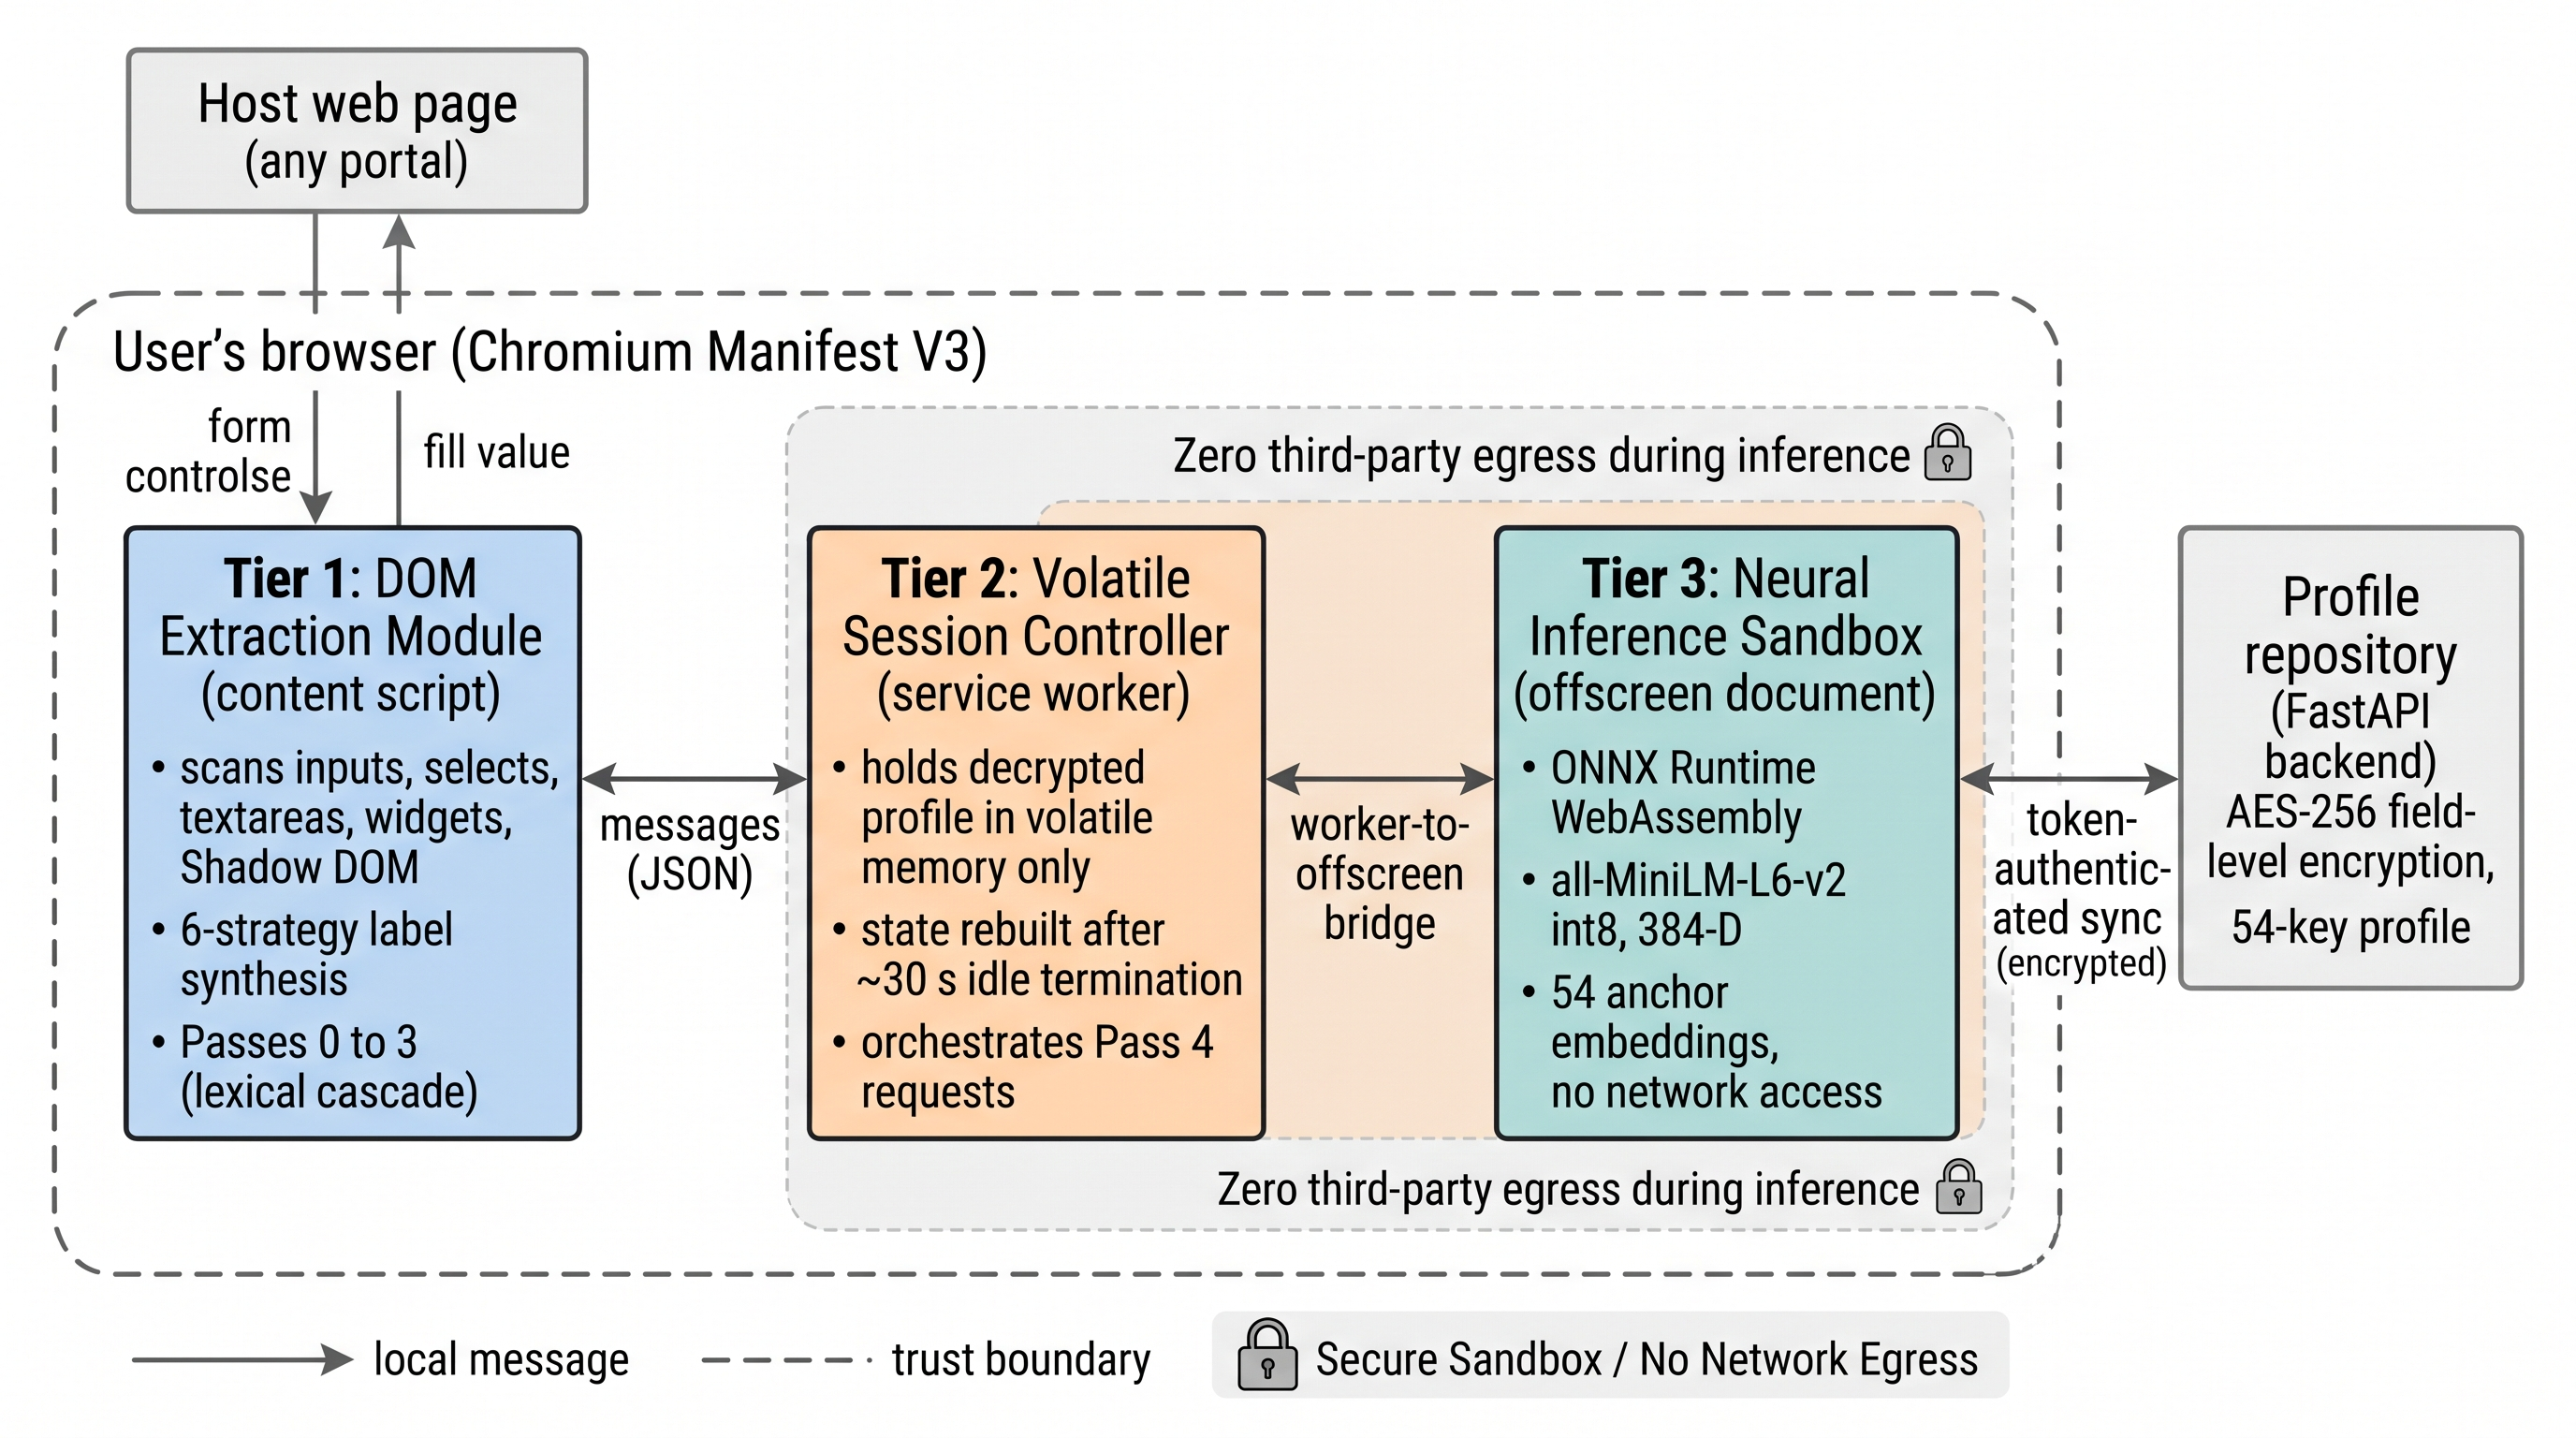
\includegraphics[width=0.98\textwidth,height=5.2cm,keepaspectratio]{fig_architecture.jpg}
\caption{GovConnect reference architecture and zero-egress neural inference boundary.}
\label{fig:arch}
\end{figure}

The decision flow of the cascade is illustrated in Fig.~\ref{fig:pipeline}:
Pass 0 (W3C Lookup): Evaluates the HTML5 \texttt{autocomplete} attribute against standard tokens (\texttt{given-name}, \texttt{email}, \texttt{tel}). Exact matches resolve deterministically in $<0.001$~ms.
Pass 1 (Prefix Stripping \& Abbreviation Expansion): Strips numeric row prefixes with regex \texttt{/\textasciicircum[0-9]+\allowbreak[\_-]*/} when at least two alphabetic characters remain (\texttt{02frstname} $\to$ \texttt{frstname}), strips vendor prefixes (\texttt{txt\_}, \texttt{ctl00\$}), and expands 29 legacy 8-character abbreviations (\texttt{pers\_ssn} $\to$ \texttt{nik}, \texttt{cellphon} $\to$ \texttt{phone}, \texttt{driv\_lic} $\to$ \texttt{driver\_license}, \texttt{workphon} $\to$ \texttt{work\_phone}).
Pass 1.5 (Option-Profiled Heuristics): Inspects option label and value distributions for unlabelled \texttt{<select>} controls. Numeric ranges $[1,31]$, $[1,12]$, and $[1900,2026]$ deterministically resolve birth day, month, and year controls.
Pass 2 (Tokenization \& Scoped Cross-Domain Vetoes): Deconstructs identifiers via camelCase and delimiter splits. To prevent false-positive cross-domain collisions, six hardcoded scoped vetoes are evaluated inline: (1) \texttt{hasIbu} prevents maternal labels from binding to the applicant name; (2) \texttt{hasAyah} vetoes applicant name for paternal fields; (3) \texttt{hasDarurat} vetoes primary phone for emergency contacts; (4) \texttt{hasKantor} / \texttt{work} vetoes home phone and residential address; (5) \texttt{hasHome} vetoes mobile phone; and (6) \texttt{hasFax} vetoes standard telephone keys.
Pass 2.5 (Query-Normalized BM25): Evaluates multi-token narrative labels where character distances degrade. BM25 scores are normalized by query token count $|Q|$ to prevent penalty on descriptive labels:
\begin{equation}
\text{Score}_{\text{BM25}}(Q, D) = \frac{1}{|Q|} \sum_{q \in Q} \frac{\text{IDF}(q) \cdot \text{TF}(q, D) \cdot (k_1 + 1)}{\text{TF}(q, D) + k_1 \cdot \left(1 - b + b \cdot \frac{|D|}{\text{avgdl}}\right)}
\end{equation}

\begin{figure}[t]
\centering
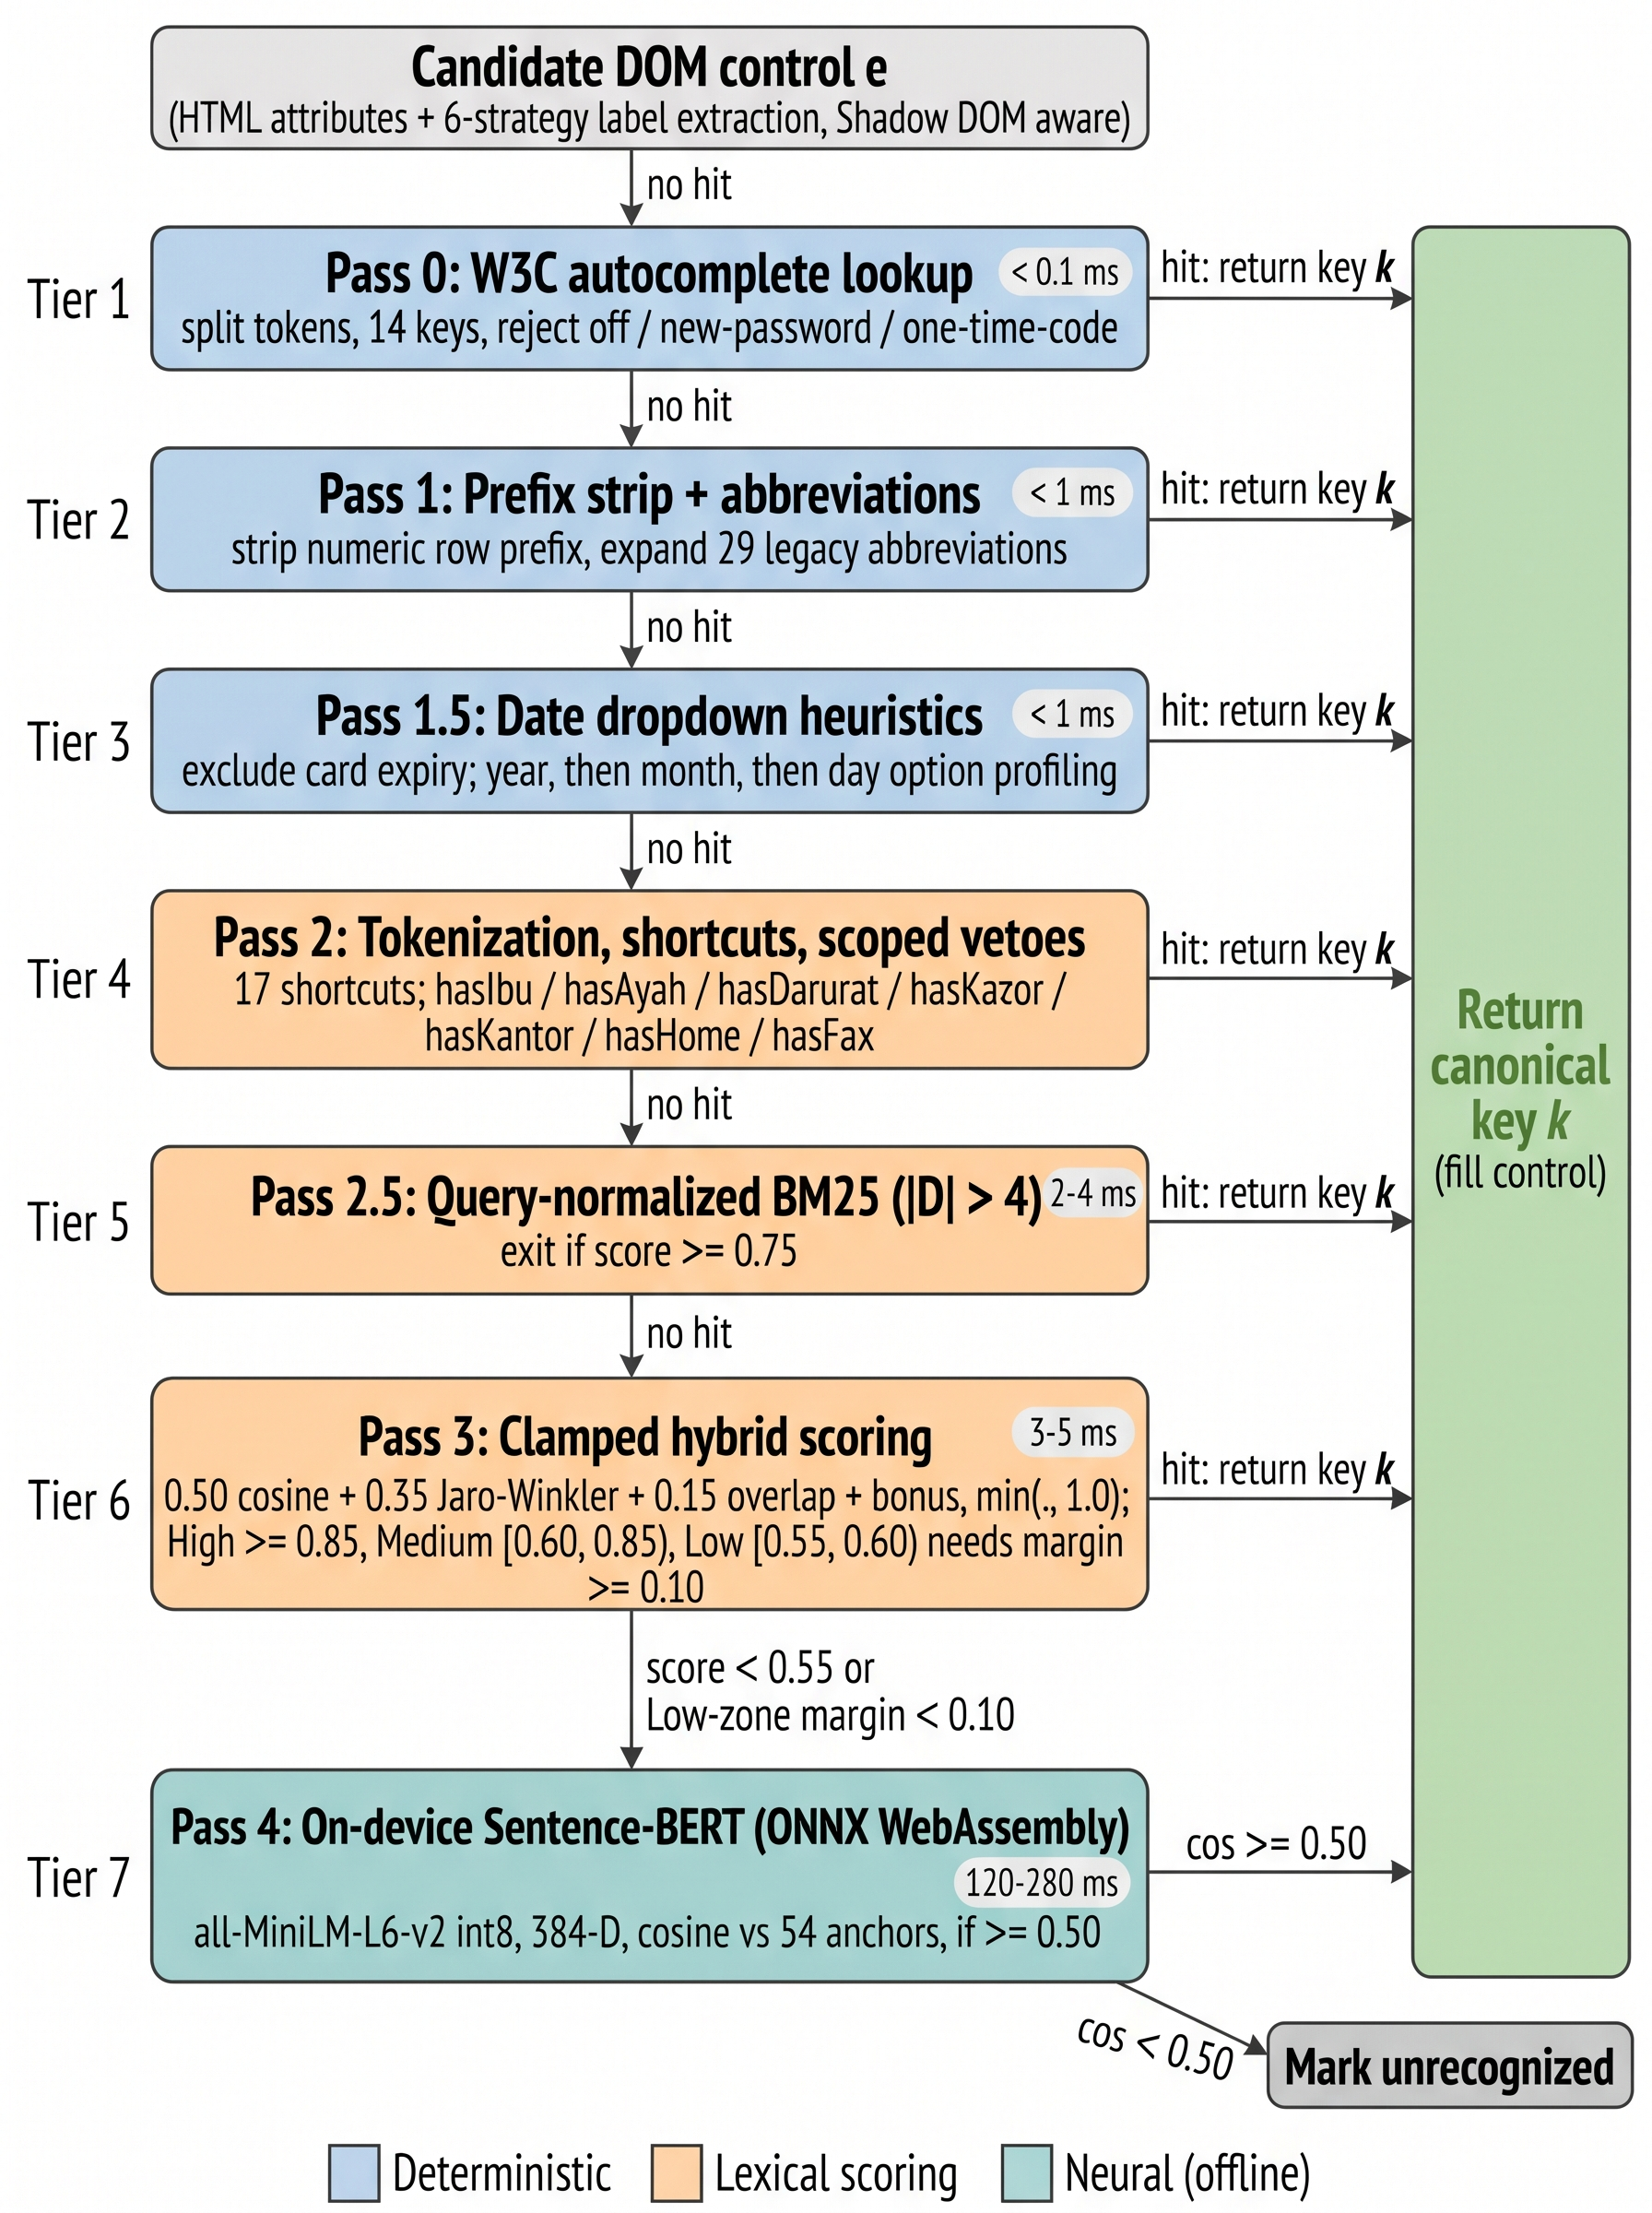
\includegraphics[width=0.75\textwidth,height=6.6cm,keepaspectratio]{fig_pipeline.jpg}
\caption{Decision flow across the seven tiers of the Hybrid Cascade Pipeline.}
\label{fig:pipeline}
\end{figure}

Parameters are calibrated to $k_1 = 1.2$, $b = 0.30$, $\text{avgdl} = 6.0$, and $\text{IDF} = 1.0$, allowing high-overlap narrative phrases to exceed the exit threshold $\tau = 0.75$.
Pass 3 (Clamped Hybrid Lexical Scoring): Evaluates a weighted linear combination of Jaro-Winkler ($\text{JW}$), substring containment ($\text{Sub}$), Levenshtein ($\text{Lev}$), and S{\o}rensen-Dice ($\text{Dice}$), with domain bonuses:
\begin{equation}
\text{Score}_{\text{final}} = \min\left(1.0, 0.40\,\text{JW} + 0.35\,\text{Sub} + 0.15\,\text{Lev} + 0.10\,\text{Dice} + \text{Bonus}\right)
\end{equation}
Confidence routing operates across three zones: High ($\ge 0.85$) and Medium ($0.60 \le s < 0.85$) accept the top candidate; Low ($0.55 \le s < 0.60$) accepts only if the candidate exceeds the runner-up by a margin $\ge 0.10$. Unmatched controls ($<0.55$) escalate to Pass 4.
Pass 4 (On-Device Neural Inference): Transmits candidate label text across a local message channel to the offscreen document hosting INT8-quantized \texttt{all-MiniLM-L6-v2} (22.7~MB). Cosine similarity between candidate embedding $\mathbf{e}_{\text{field}}$ and target profile embeddings $\mathbf{e}_{\text{target}}$ is evaluated. As verified in the reference codebase, Pass 4 executes without a margin guard, resolving controls exceeding a fixed threshold of 0.50.

\section{Experimental Evaluation}
We evaluated the pipeline across 5 live English-language reference pages representing all four heterogeneity classes ($N = 177$ DOM controls inspected): RoboForm All-Fields ($N = 41$, Class 2 legacy abbreviations), University of Michigan Wolverine Access ($N = 54$, Class 1 W3C and Class 3 components), SelectorsHub Practice Form ($N = 41$, Class 3 modern frameworks and security traps), GetAutoClicker ($N = 22$, Class 1/2 mixed controls), and PasswordManager UK ($N = 19$, Class 3 obfuscated \texttt{textfield*} controls). We annotated 64 target controls corresponding to canonical user profile keys using a standardized single-annotator codebook.

\begin{table}[t]
\caption{Measured performance comparison across 64 annotated target controls.}
\label{tab:baseline}
\centering
\scriptsize
\setlength{\tabcolsep}{4.5pt}
\begin{tabular}{p{3.2cm}cccc}
\toprule
\textbf{Architecture / Baseline} & \textbf{Resolved} & \textbf{Recall [95\% CI]} & \textbf{Prec.} & \textbf{Mean Latency} \\
\midrule
Native Chromium autofill~\cite{chromium} & 38/64 & 59.4\% [47.1, 70.5] & 100.0\% & 0.011 ms \\
TF-IDF + logistic regression & 48/64 & 75.0\% [63.2, 84.0] & 98.0\% & 0.664 ms \\
Rule-only (Pass 0--1.5) & 36/64 & 56.3\% [44.1, 67.8] & 100.0\% & $<0.001$ ms \\
\textbf{Hybrid Cascade Pipeline} & \textbf{62/64} & \textbf{96.9\%} [89.3, 99.1] & \textbf{100.0\%} & \textbf{$<5$ ms (95.3\%)$^{*}$} \\
=======
\begin{center}
{\fontsize{13.5}{16}\selectfont\bfseries A Resource-Efficient Hybrid Cascade Pipeline for Client-Side Schema Matching of Heterogeneous Web Forms with On-Device Sentence-BERT\par}

\vspace{5pt}
{\normalsize\normalfont Andharu Raffi$^1$, Fajrian Aprilio$^1$, Amma Liesvarastranta Haz$^{1\,[0000-0002-5612-6062]}$, Evianita Dewi Fajrianti$^{1\,[0000-0002-9019-9775]}$, and Sritrusta Sukaridhoto$^{1\,[0000-0002-8157-5863]}$\par}

\vspace{3.5pt}
{\small\normalfont
$^1$ Department of Informatics and Computer Engineering, Politeknik Elektronika Negeri Surabaya, Surabaya, Indonesia\\
\texttt{liesvarastranta@pens.ac.id}\par}
\end{center}

\vspace{2pt}
\begin{quote}
\small\normalfont
\noindent\textbf{Abstract.} Filling personal attributes into heterogeneous web forms is an instance of schema matching, where the source schema is a user profile and the target schema is an unseen set of form controls. Rule-only matchers fail on non-cognate and opaque identifiers, while cloud LLM matchers add network latency, recurring per-token cost, and data residency exposure. This paper proposes the Hybrid Cascade Pipeline, a resource-efficient client-side matching algorithm that escalates each control through seven tiers: W3C \texttt{autocomplete} lookup, prefix stripping with legacy abbreviation expansion, option-profiled date heuristics, tokenization with scoped cross-domain vetoes, query-normalized BM25 ranking, clamped hybrid lexical scoring with a runner-up margin guard, and on-device Sentence-BERT inference over quantized ONNX WebAssembly. The algorithm is implemented in \emph{GovConnect}, a proof-of-concept Chromium Manifest V3 extension testbed. Across 313 inspected controls (177 English reference controls, 64 annotated targets; 136 live Indonesian controls), the pipeline resolves 62 of 64 target controls (96.9\% recall; 95\% Wilson CI $[89.3\%, 99.1\%]$), compared with 59.4\% for native Chromium autofill, 75.0\% for a TF-IDF logistic regression baseline, and 56.3\% for rule-only matching. Over 95\% of target controls resolve on a fast lexical path below 5~ms. All 63 security/credential traps were safely rejected (0.0\% FPR). A supplementary evaluation on 5 Indonesian public portals confirmed 41/41 (100\%) core identity resolution, and a white-box readiness audit delineates operational boundary conditions.

\vspace{2pt}
\noindent\textbf{Keywords:} Schema Matching $\cdot$ Hybrid Cascade Pipeline $\cdot$ Form Resolution $\cdot$ Client-Side Edge AI $\cdot$ Sentence-BERT $\cdot$ Privacy by Design.
\end{quote}

\section{Introduction}
\noindent Public administrations and enterprises operate thousands of web portals, from tax and civil registration services to academic platforms. Backend interoperability programs intended to harmonize cross-agency data exchange are widely reported as slow, costly, and hampered by multi-vendor coordination, as in the Indonesian electronic-based government system (SPBE) under Presidential Regulation No.~95/2018 \cite{hermanto2022,spbe2018}. Where backend exchange is unavailable, users must repeatedly retype identical identity, contact, and demographic attributes into fragmented forms.

Automatic form resolution is an applied instance of schema matching: each form control must be mapped to one canonical profile key. The task is harder than standardized e-commerce checkout forms covered by HTML \texttt{autocomplete} \cite{whatwg2026}, because real-world portals span four structural heterogeneity classes: (1) standards-compliant HTML5 controls; (2) legacy ASP, JSP, and ERP modules with truncated 8-character identifiers and numeric row prefixes (\texttt{02frstname}, \texttt{23cellphon}); (3) single-page applications and table layouts with opaque identifiers (\texttt{input-7a9f}, \texttt{textfield23}); and (4) verbose narrative labels without technical attribute clues.

Deterministic pattern matching frequently fails on non-cognate synonyms, such as \texttt{05\_company} for \texttt{organization} or \texttt{14adrstate} for \texttt{province}. While Large Language Models (LLMs) can resolve these semantic discrepancies, delegating form resolution to remote cloud endpoints introduces significant engineering and regulatory hurdles. In particular, transmitting page structures and sensitive user attributes across network boundaries incurs noticeable latency ($1.5\text{--}4.0\text{ s}$ per form request), recurring token costs, and potential non-compliance with data residency mandates under Indonesia's PDP Law (UU No.~27/2022) \cite{pdp2022} and the EU GDPR \cite{gdpr2016}.

This paper treats form resolution as an algorithmic schema matching problem and investigates a complementary client-side layer. We formulate three research questions:
\begin{itemize}
    \item \textbf{(RQ1)} How accurately can a hierarchical lexical-to-neural cascade resolve non-cognate and obfuscated controls without cloud LLM inference?
    \item \textbf{(RQ2)} Does the cascade operate within interactive browser latency budgets?
    \item \textbf{(RQ3)} What privacy boundary can be enforced during inference, and which boundary conditions remain open under a white-box readiness audit?
\end{itemize}

The main contributions of this study are as follows: (1) the Hybrid Cascade Pipeline, a seven-tier matching algorithm combining deterministic lookup, scoped cross-domain vetoes, query-normalized BM25, clamped hybrid scoring, and offline quantized Sentence-BERT; (2) an empirical evaluation on 5 English benchmark websites (177 controls inspected, 64 annotated target controls) against three measured baselines and a per-tier ablation, supplemented by a test on 5 Indonesian portals ($N = 136$ controls; 313 total inspected); and (3) a readiness and threat analysis of the GovConnect reference implementation.

\section{Related Work}
\noindent Automatic schema matching maps elements between heterogeneous source and target schemas \cite{rahm2001,koutras2021}. Empirical benchmarks by Koutras et al.\ \cite{koutras2021} demonstrate that while lexical comparators (such as Jaro-Winkler and token overlap) excel on syntactic variants, combining complementary matchers is essential when surface forms diverge. In web environments, native browser autofill relies on static regular expression dictionaries and standardized W3C \texttt{autocomplete} tokens \cite{whatwg2026,chromium2024}. However, recent security audits by Fu and Wang \cite{fu2024} reveal that indiscriminate browser and password-manager autofill frequently misclassifies hidden or ambiguous form traps, motivating stricter scoped vetoes and negative-trap filtering.

To resolve non-cognate attributes without manual feature engineering, recent studies have adopted pre-trained language models (PLMs) and foundation models for schema matching and data wrangling \cite{zhang2023,parciak2024,narayan2022}. Zhang et al.\ \cite{zhang2023} and Parciak et al.\ \cite{parciak2024} show that transformer-based representations effectively capture semantic correspondence across disparate column names, though querying hosted LLMs incurs substantial latency and verification overhead \cite{parciak2024,narayan2022}. At the edge, Sentence-BERT (SBERT) \cite{reimers2019} and distilled architectures such as MiniLM \cite{wang2020} enable compact dense embeddings. Recent advances in WebAssembly (WASM) runtime optimization have made in-browser deep learning inference viable on commodity client CPUs \cite{jia2024}, allowing our cascade to combine fast lexical filtering with local neural inference without external data egress.

\section{The Hybrid Cascade Pipeline}
\noindent The GovConnect reference architecture (Fig.~\ref{fig:arch}) executes as a Manifest V3 Chromium extension comprising two execution boundaries: a content script executing directly within the host DOM, and a sandboxed offscreen document hosting ONNX Runtime WebAssembly. The matching engine evaluates candidate form controls against a canonical schema of 45 personal, contact, and educational attributes through a seven-tier escalation cascade. The decision flow of the cascade is illustrated in Fig.~\ref{fig:pipeline}.

\begin{figure}[!t]
\centering
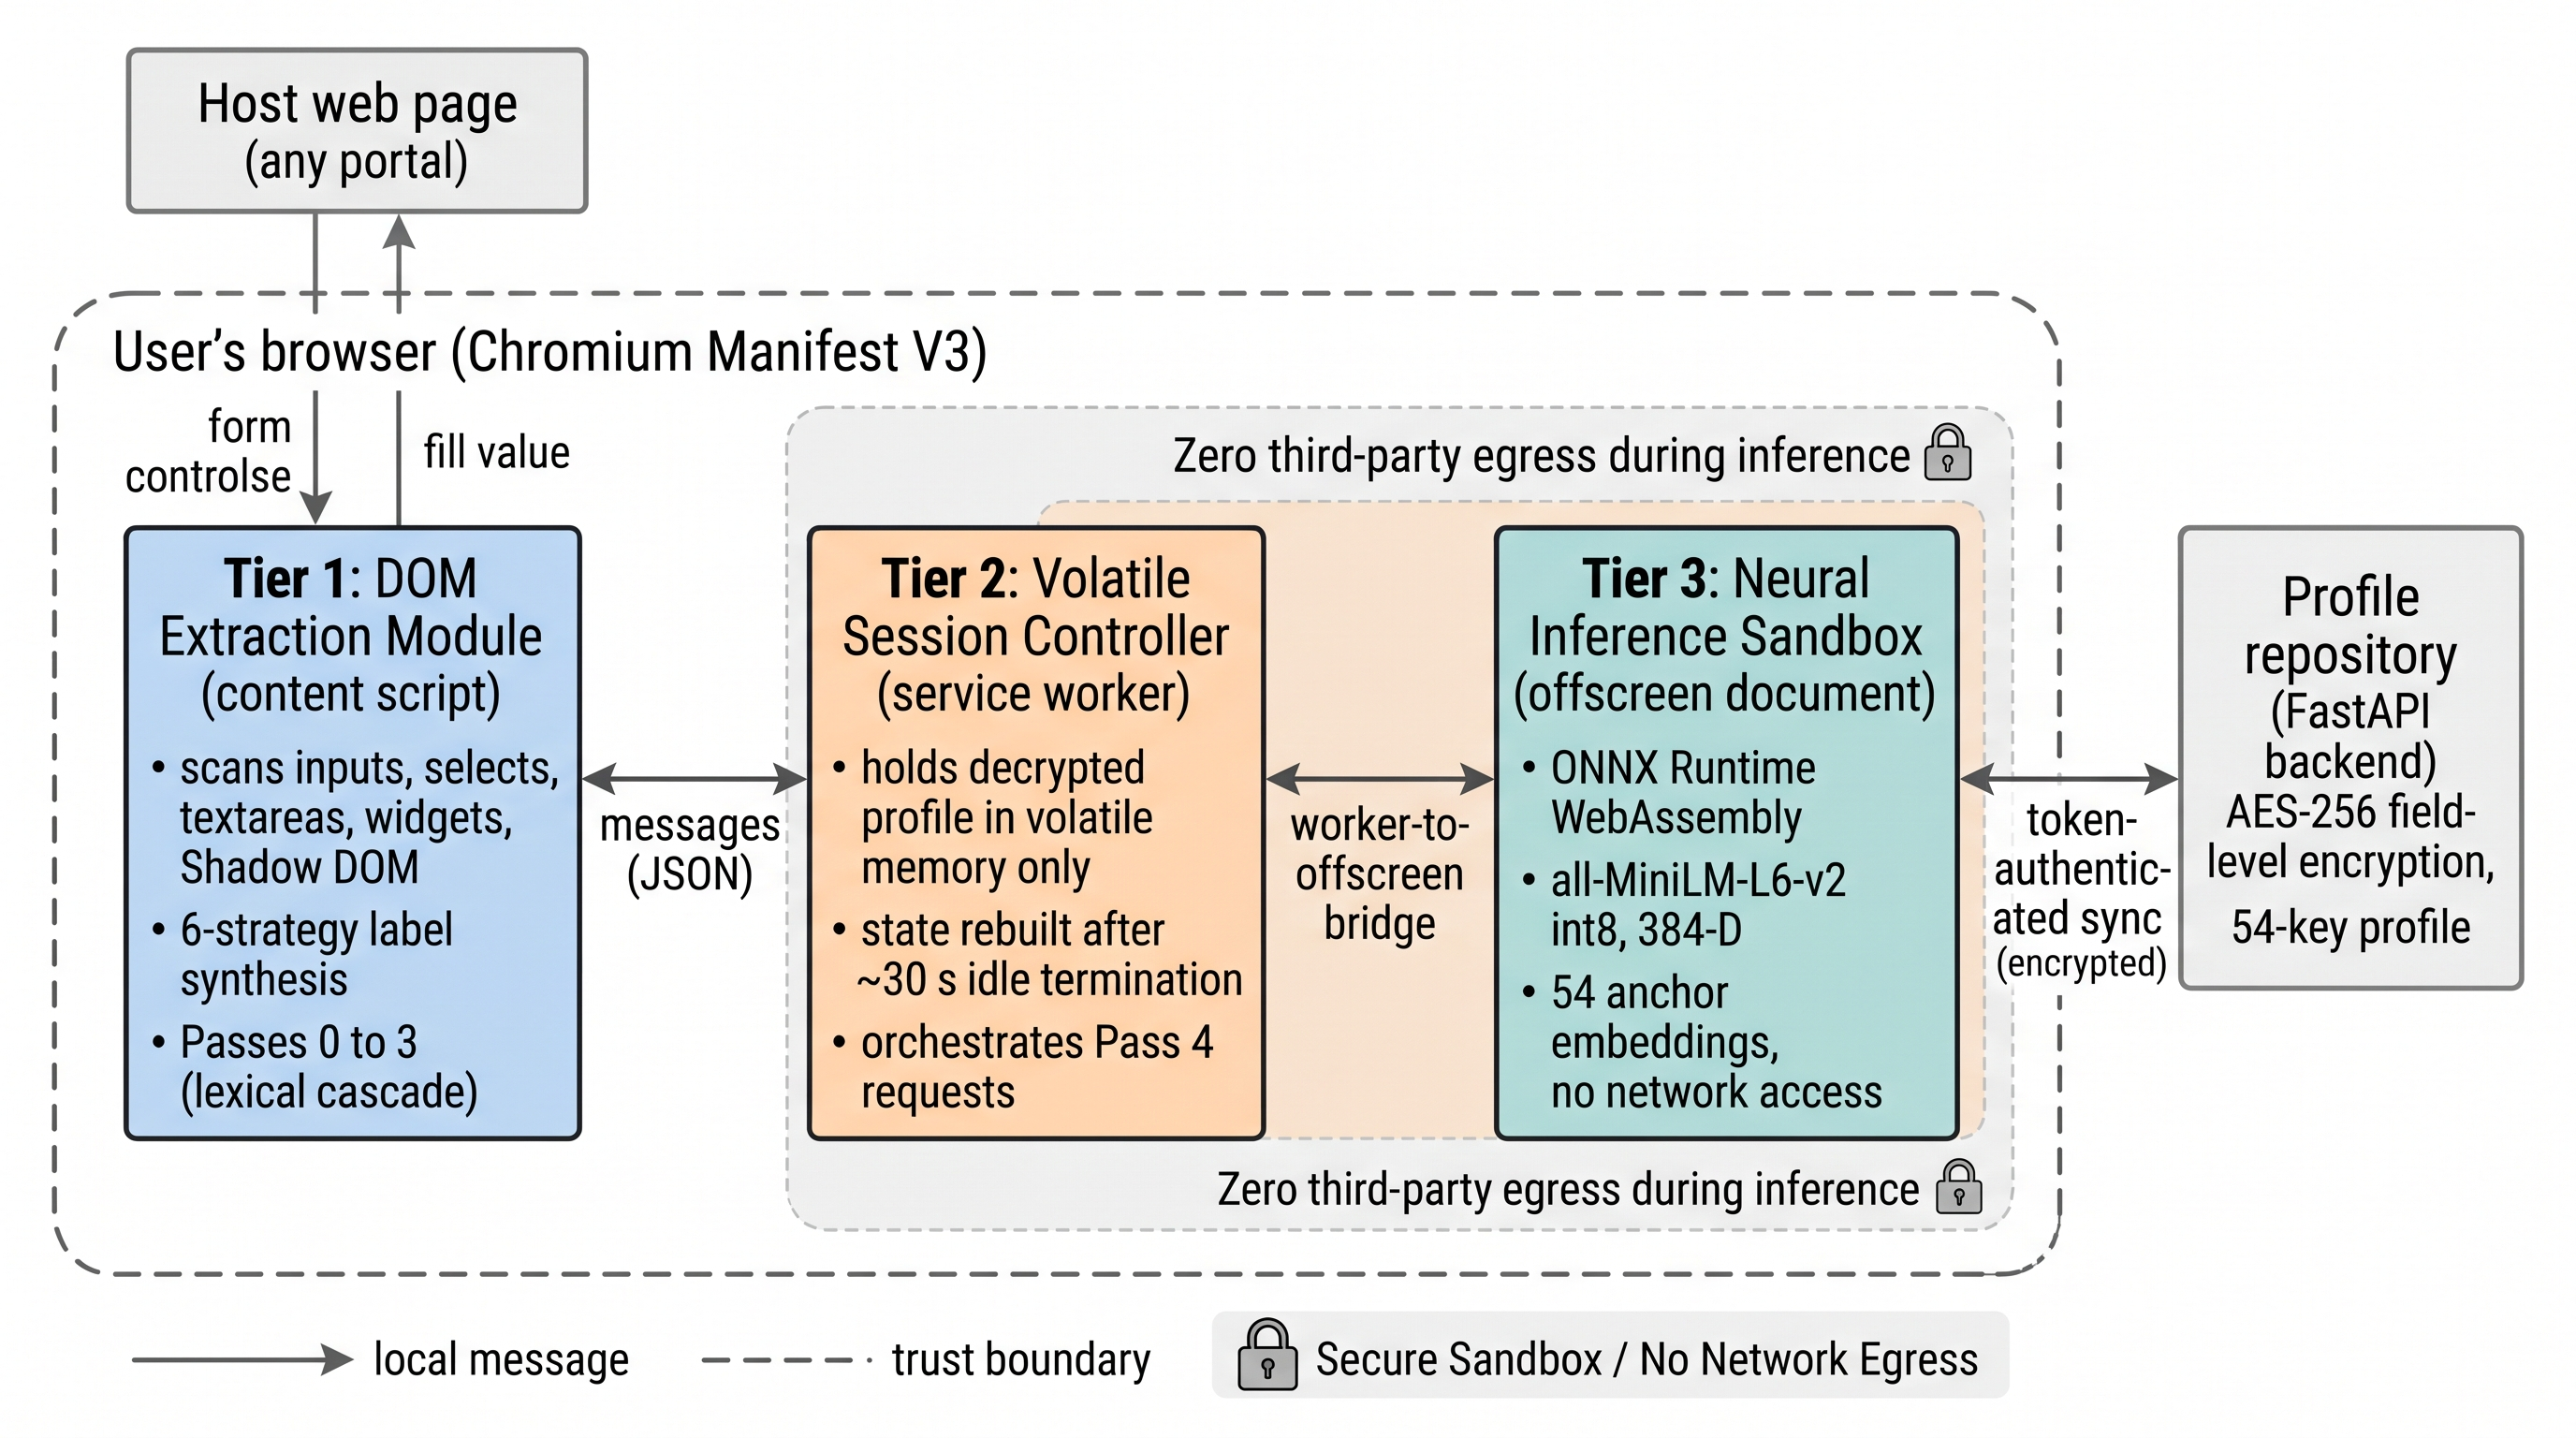
\includegraphics[width=\textwidth]{fig1_architecture.jpg}
\lncsfigcaption{GovConnect reference architecture and zero-egress neural inference boundary.}
\label{fig:arch}
\end{figure}

In Pass~0 (W3C Lookup), the engine evaluates the HTML5 \texttt{autocomplete} attribute against standard tokens (\texttt{given-name}, \texttt{email}, \texttt{tel}). Exact matches resolve deterministically in $<0.001$~ms while ignoring non-identity tokens (\texttt{off}, \texttt{new-password}, \texttt{one-time-code}).

Subsequently, Pass~1 (Prefix Stripping and Abbreviation Expansion) strips numeric row prefixes with regex \texttt{/\^{}[0-9]+[\_-]*/} when at least two alphabetic characters remain (\texttt{02frstname} $\rightarrow$ \texttt{frstname}), strips vendor prefixes (\texttt{txt\_}, \texttt{ctl00\$}), and expands 29 legacy 8-character abbreviations (\texttt{pers\_ssn} $\rightarrow$ \texttt{nik}, \texttt{cellphon} $\rightarrow$ \texttt{phone}, \texttt{driv\_lic} $\rightarrow$ \texttt{driver\_license}, \texttt{workphon} $\rightarrow$ \texttt{work\_phone}) against canonical alias sets.

For unlabelled \texttt{<select>} controls, Pass~1.5 (Option-Profiled Heuristics) inspects option label and value distributions. Numeric ranges $[1, 31]$, $[1, 12]$, and $[1900, 2026]$ deterministically resolve birth day, month, and year controls while excluding payment card expiry fields (\texttt{ccexp}).

In Pass~2 (Tokenization and Scoped Cross-Domain Vetoes), identifiers are deconstructed via camelCase and delimiter splits. To prevent false-positive cross-domain collisions, six hardcoded scoped vetoes are evaluated inline (Table~\ref{tab:veto}): (1) \texttt{hasIbu} prevents maternal labels from binding to the applicant name; (2) \texttt{hasAyah} vetoes applicant name for paternal fields; (3) \texttt{hasDarurat} vetoes primary phone for emergency contacts; (4) \texttt{hasKantor} / \texttt{work} vetoes home phone and residential address; (5) \texttt{hasHome} vetoes mobile phone; and (6) \texttt{hasFax} vetoes standard telephone keys.

\begin{figure}[!t]
\centering
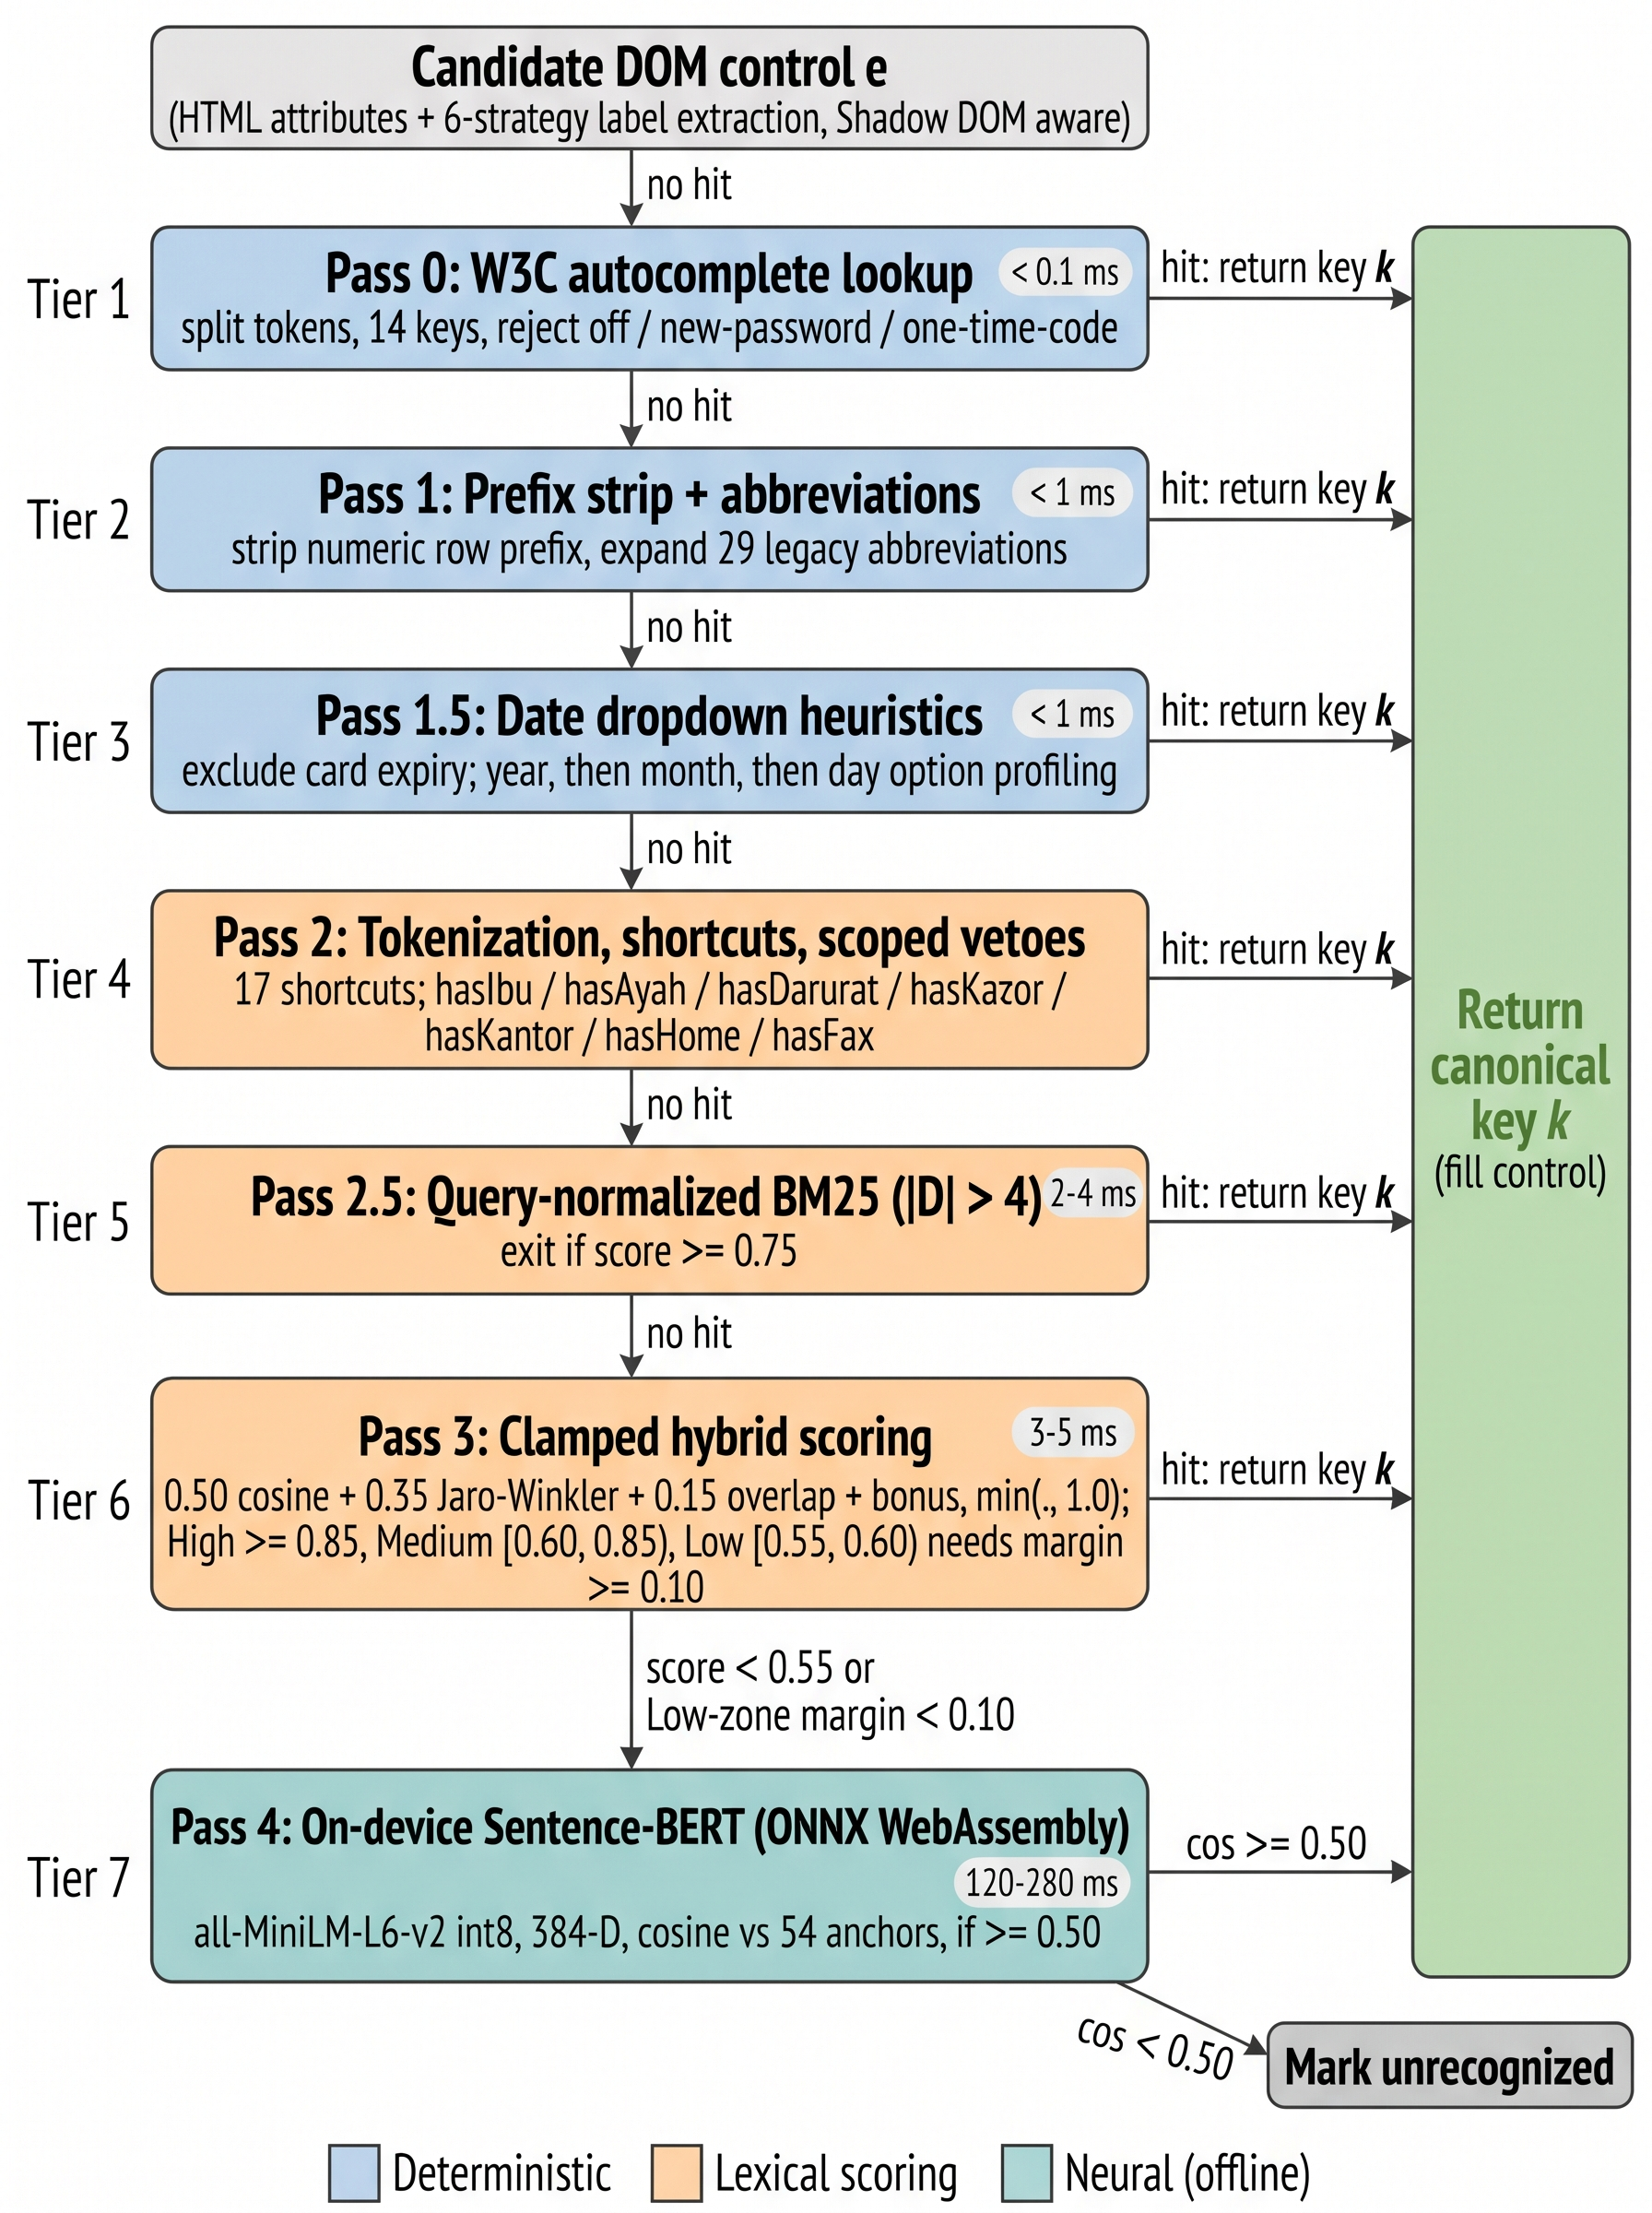
\includegraphics[width=\textwidth]{fig2_decision_flow.jpg}
\lncsfigcaption{Decision flow across the seven tiers of the Hybrid Cascade Pipeline. Parameters are calibrated to: $k_1 = 1.2$, $b = 0.30$, $\text{avgdl} = 6.0$, and $\text{IDF} = 1.0$, allowing high-overlap narrative phrases to exceed the exit threshold $\gamma = 0.75$.}
\label{fig:pipeline}
\end{figure}

\begin{table}[!t]
\lncstablecaption{Scoped cross-domain veto rules and context modifiers in Pass 2 and Pass 3.}
\label{tab:veto}
\scriptsize\normalfont
\setlength{\tabcolsep}{3.5pt}
\renewcommand{\arraystretch}{0.95}
\begin{tabularx}{\textwidth}{L{2.5cm}L{2.2cm}L{2.8cm}Y}
\toprule
\textbf{Trigger Tokens in $D$} & \textbf{Modifier Flag} & \textbf{Scoped Veto Target} & \textbf{Redirected Target \& Pass 3 Bonus} \\
\midrule
\texttt{"ibu"}, \texttt{"mother"} & \texttt{hasIbu = true} & Veto personal \texttt{full\_name} & Redirects to \texttt{mother\_name} ($+0.25$ bonus) \\
\texttt{"ayah"}, \texttt{"father"} & \texttt{hasAyah = true} & Veto personal \texttt{full\_name} & Redirects to \texttt{father\_name} ($+0.25$ bonus) \\
\texttt{"darurat"}, \texttt{"emergency"} & \texttt{hasDarurat = true} & Veto personal \texttt{full\_name} \& \texttt{phone} & Redirects to \texttt{emergency\_contact\_*} ($+0.30$) \\
\texttt{"kantor"}, \texttt{"office"} & \texttt{hasKantor = true} & Veto domicile \texttt{address} & Redirects to \texttt{work\_address} ($+0.25$ bonus) \\
\texttt{"rumah"}, \texttt{"home"} & \texttt{hasHome = true} & Veto mobile/work phone only & Redirects to \texttt{home\_phone} ($+0.35$; preserves \texttt{address}) \\
\texttt{"fax"}, \texttt{"telefax"} & \texttt{hasFax = true} & Veto all voice phone keys & Redirects exclusively to \texttt{fax} ($+0.40$ bonus) \\
>>>>>>> 22dced0dec94ea2987d8bfef8029690236ebd8f5
\bottomrule
\multicolumn{5}{l}{\tiny $^{*}$Lexical tiers (Pass 0--3) resolve in $<5$ ms; Pass 4 neural inference requires 120--280 ms on client CPU.}
\end{tabular}
\end{table}

<<<<<<< HEAD
Table~\ref{tab:baseline} compares the pipeline against three baselines: (1) native Chromium autofill heuristics~\cite{chromium}; (2) a TF-IDF character and word n-gram logistic regression classifier trained on form corpora; and (3) a rule-only matcher (Pass 0--1.5). The Hybrid Cascade Pipeline resolved 62 of 64 target controls (96.9\% recall; Wilson 95\% CI [89.3\%, 99.1\%]), significantly outperforming Chromium autofill (59.4\%) and the statistical classifier (75.0\%).

A rigorous accounting of all 177 inspected DOM controls shows: (1) 64 annotated target controls; (2) 26 auxiliary identity/demographic controls (e.g. secondary address lines, country prefixes, application notes) not present in the minimal canonical profile; (3) 63 security/credential/payment traps (passwords, PINs, card numbers, CVVs, CAPTCHAs, hidden CSRF tokens), including 6 traps on SelectorsHub; the pipeline achieved 100\% true negative rejection (63/63, 0.0\% FPR); and (4) 24 UI widget fallbacks (unlabelled checkboxes, radio toggles).

\begin{table}[t]
\caption{Resolution of 10 non-name attribute categories across 5 benchmark sites.}
\label{tab:cat}
\centering
\scriptsize
\setlength{\tabcolsep}{4pt}
\begin{tabular}{l l c c c c c}
\toprule
\textbf{Category} & \textbf{Observed Lexical Variants} & \textbf{Robo} & \textbf{UMich} & \textbf{Hub} & \textbf{Auto} & \textbf{Pass} \\
\midrule
Address line & \texttt{adr\_address1}, \texttt{address}, \texttt{street} & 1/1 & 2/2 & 1/1 & 1/1 & 1/1 \\
City & \texttt{adr\_city}, \texttt{city}, \texttt{town} & 1/1 & 1/1 & 1/1 & -- & 1/1 \\
State / Prov. & \texttt{adr\_state}, \texttt{14adrstate}, \texttt{state} & 1/1 & 1/1 & 1/1 & -- & 1/1 \\
ZIP / Postcode & \texttt{adr\_zipcode}, \texttt{zip}, \texttt{postal-code} & 1/1 & 1/1 & 1/1 & -- & 1/1 \\
Country & \texttt{adr\_country}, \texttt{country}, \texttt{country-name} & 1/1 & 1/1 & 1/1 & -- & 1/1 \\
Email & \texttt{04\_email}, \texttt{email}, \texttt{userEmail} & 1/1 & 1/1 & 1/1 & 1/1 & 1/1 \\
Phone & \texttt{23cellphon}, \texttt{homephon}, \texttt{mobile} & 4/4 & 3/3 & 1/1 & 1/1 & 2/2 \\
Birth date & \texttt{66mm/67dd/68yy}, \texttt{bday-*}, \texttt{dob} & 3/3 & 3/3 & 1/1 & 1/1 & 1/1 \\
Gender & \texttt{gender}, \texttt{sex}, \texttt{opt\_gender} & 1/1 & 1/1 & 1/1 & -- & -- \\
Organization & \texttt{05\_company}, \texttt{organization}, \texttt{firm} & 1/1 & 1/1 & 1/1 & -- & 1/1 \\
\midrule
\textbf{Site Total} & & \textbf{18/18} & \textbf{18/19} & \textbf{10/11} & \textbf{4/4} & \textbf{12/12} \\
\bottomrule
\end{tabular}
\end{table}

Table~\ref{tab:cat} presents category-level resolution across the benchmark sites. The cumulative ablation demonstrates the efficiency of cascading tiers: Pass 0 resolves 28.1\% (18/64); Pass 1 and 1.5 expand resolution to 56.3\% (36/64); Pass 2 reaches 87.5\% (56/64) via scoped vetoes; Pass 2.5 and 3 resolve 95.3\% (61/64) on fast lexical paths ($<5$~ms); and Pass 4 neural inference recovers the final ambiguous control (\texttt{104\_other\_income} $\to$ \texttt{annual\_income}, cosine 0.54) to attain 96.9\% (62/64).

Cross-jurisdictional generalization was verified across 5 live Indonesian portals ($N = 136$ DOM controls; 313 total): Coretax DJP (47), SMK Semen Gresik admission (31), SSCASN BKN civil recruitment (28), a localized civil registration form on JotForm replicating Indonesian Population and Civil Registration (Dukcapil -- \emph{Kependudukan dan Pencatatan Sipil}) workflows (21), and OSS BKPM licensing (9). Across 41 core identity controls (7 on Coretax, 11 on SSCASN, 2 on OSS, 6 on SMK, 15 on JotForm), the pipeline resolved 41/41 (100\%), reaching 98/99 (99.0\%) core identity recall combined with the English suite.

\section{Discussion: Practicality, Privacy, and Readiness}
From a practical deployment standpoint, client-side schema matching offers an immediately deployable bridge over administrative fragmentation. Executing as an unprivileged browser extension within the user agent, GovConnect operates on live legacy and modern public portals without requiring backend code changes, multi-vendor coordination, or database synchronization. The operational footprint is exceptionally compact: the INT8-quantized MiniLM model requires 22.7~MB of memory and executes fully offline via WebAssembly~\cite{onnxweb,transformersjs}. Over 95\% of form controls resolve deterministically or lexically in $<5$~ms, reserving neural inference exclusively for sparse non-cognate ambiguities.

In terms of data governance, client-side inference enforces a strict privacy perimeter. Offloading form parsing to hosted LLM APIs risks transmitting sensitive citizen attributes across network boundaries. GovConnect confines ONNX WebAssembly inference to an isolated offscreen document lacking network socket permissions, ensuring a zero-egress boundary during matching. This architecture fulfills Data Protection by Design and by Default under GDPR Article 25~\cite{gdpr} and complies with statutory data residency mandates under Indonesia's PDP Law (UU No.~27/2022)~\cite{uupdp}.

\begin{table}[t]
\caption{Boundary conditions and readiness status of the reference implementation.}
\label{tab:audit}
\centering
\scriptsize
\setlength{\tabcolsep}{3pt}
\renewcommand{\arraystretch}{0.90}
\begin{tabular}{p{2.0cm}p{2.8cm}p{1.4cm}p{5.1cm}}
\toprule
\textbf{Component Tier} & \textbf{Boundary Condition} & \textbf{Status} & \textbf{Architectural Resolution / Roadmap} \\
\midrule
Pass 3 Scoring & Unbounded score ($\sim$1.40) & Resolved & Clamped with $\min(\cdot)$; margin guard on $[0.55,0.60)$ \\
Pass 2.5 BM25 & Cap of 0.52 made tier inactive & Recalibrated & $b{=}0.30$, $\text{avgdl}{=}6.0$, $\tau{=}0.75$; corpus IDF planned \\
DOM Injection & Silent overwrite \& desync & Identified & Post-fill check (\texttt{el.value===target}) and overwrite guard \\
Pass 4 Neural & Monolingual, uncalibrated 0.50 & Roadmap & Multilingual SBERT, ROC calibration, margin guard \\
Form Layout & Joint controls (\texttt{ttl} place+date) & Roadmap & Bipartite assignment, proximity header parsing \\
=======
When narrative labels exceed four tokens, Pass~2.5 (Query-Normalized BM25) evaluates multi-token relevance where character distances degrade. BM25 scores \cite{robertson2009} are normalized by query token count $|Q|$ to prevent penalty on descriptive labels:
\begin{equation}
\text{Score}_{\text{BM25}}(Q, D) = \min\!\left(\frac{1}{|Q| \cdot \gamma} \sum_{q \in Q \cap D} \text{IDF}(q) \cdot \frac{\text{TF}(q, D) \cdot (k_1 + 1)}{\text{TF}(q, D) + k_1 \cdot \left(1 - b + b \cdot \frac{|D|}{\text{avgdl}}\right)},\; 1.0\right)
\label{eq:bm25}
\end{equation}

Candidates remaining unresolved enter Pass~3 (Clamped Hybrid Lexical Scoring), which evaluates a weighted linear combination of Jaro-Winkler ($\text{JW}$), substring containment ($\text{Sub}$), Levenshtein ($\text{Lev}$), and S{\o}rensen-Dice ($\text{Dice}$), with domain context bonuses:
\begin{equation}
\text{Score}_{\text{final}} = \min\!\left(0.40\,\text{JW} + 0.35\,\text{Sub} + 0.15\,\text{Lev} + 0.10\,\text{Dice} + \text{Bonus},\; 1.0\right)
\label{eq:hybrid}
\end{equation}
Confidence routing operates across three zones: High ($\ge 0.85$) and Medium ($[0.60, 0.85)$) accept the top candidate; Low ($[0.55, 0.60)$) accepts only if the candidate exceeds the runner-up by a margin $\ge 0.10$. Unmatched controls ($<0.55$) escalate to Pass~4.

Finally, Pass~4 (On-Device Neural Inference) transmits candidate label text across a local message channel to the offscreen document hosting INT8-quantized \texttt{all-MiniLM-L6-v2} (22.7~MB) \cite{reimers2019,wang2020}. Cosine similarity between candidate embedding $e_{\text{field}}$ and target profile embeddings $e_{\text{target}}$ is evaluated. In the reference codebase, Pass~4 executes without a margin guard, resolving controls exceeding a fixed threshold of 0.50.

\section{Experimental Evaluation}
\noindent We evaluated the pipeline across 5 live English-language reference pages representing all four heterogeneity classes ($N = 177$ DOM controls inspected): RoboForm All-Fields ($N = 41$, Class 2 legacy abbreviations), University of Michigan Wolverine Access ($N = 54$, Class 1 W3C and Class 3 components), SelectorsHub Practice Form ($N = 41$, Class 3 modern frameworks and security traps), GetAutoClicker ($N = 22$, Class 1/2 mixed controls), and PasswordManager UK ($N = 19$, Class 3 obfuscated \texttt{textfield*} controls). We annotated 64 target controls corresponding to canonical user profile keys using a standardized single-annotator codebook.

\begin{table}[!t]
\lncstablecaption{Measured performance comparison across 64 annotated target controls.}
\label{tab:comparison}
\scriptsize\normalfont
\setlength{\tabcolsep}{3.5pt}
\renewcommand{\arraystretch}{0.95}
\begin{tabularx}{\textwidth}{L{3.8cm}C{1.8cm}C{2.4cm}C{1.4cm}Y}
\toprule
\textbf{Architecture / Baseline} & \textbf{Resolved} & \textbf{Recall [95\% CI]} & \textbf{Prec.} & \textbf{Mean Latency} \\
\midrule
Native Chromium autofill \cite{chromium2024} & 38/64 & 59.4\% [47.1, 70.5] & 100.0\% & 0.011~ms \\
TF-IDF + logistic regression & 48/64 & 75.0\% [63.2, 84.0] & 98.0\% & 0.664~ms \\
Rule-only (Pass 0--1.5) & 36/64 & 56.3\% [44.1, 67.8] & 100.0\% & $<0.001$~ms \\
\textbf{Hybrid Cascade Pipeline} & \textbf{62/64} & \textbf{96.9\% [89.3, 99.1]} & \textbf{100.0\%} & \textbf{$<5$~ms (95.3\%)$^*$} \\
\bottomrule
\end{tabularx}
\vspace{1pt}
{\tiny\normalfont $^*$Lexical tiers (Pass 0--3) resolve in $<5$~ms; Pass 4 neural inference requires 120--280~ms on client CPU.\par}
\end{table}

Table~\ref{tab:comparison} compares the pipeline against three baselines: (1) native Chromium autofill heuristics \cite{chromium2024}; (2) a TF-IDF character and word n-gram logistic regression classifier trained on form corpora; and (3) a rule-only matcher (Pass 0--1.5). The Hybrid Cascade Pipeline resolved 62 of 64 target controls (96.9\% recall; Wilson 95\% CI $[89.3\%, 99.1\%]$), significantly outperforming Chromium autofill (59.4\%) and the statistical classifier (75.0\%).

A rigorous accounting of all 177 inspected DOM controls shows: (1) 64 annotated target controls; (2) 26 auxiliary identity/demographic controls (e.g., secondary address lines, country prefixes, application notes) not present in the minimal canonical profile, of which 25/26 (96.2\%) resolved accurately; (3) 63 security/credential/payment traps (passwords, PINs, card numbers, CVVs, CAPTCHAs, hidden CSRF tokens), including 6 traps on SelectorsHub, where the pipeline achieved 100\% true negative rejection (63/63, 0.0\% FPR); and (4) 24 UI widget fallbacks (unlabelled checkboxes, radio toggles).

\begin{table}[!t]
\lncstablecaption{Resolution of 10 non-name attribute categories across 5 benchmark sites.}
\label{tab:empirical_eval}
\scriptsize\normalfont
\setlength{\tabcolsep}{2.5pt}
\renewcommand{\arraystretch}{0.95}
\begin{tabularx}{\textwidth}{L{2.0cm}Y ccccc c}
\toprule
\textbf{Category} & \textbf{Observed Lexical Variants} & \textbf{Robo} & \textbf{UMich} & \textbf{Hub} & \textbf{Auto} & \textbf{Pass} & \textbf{Total} \\
\midrule
Address line & \texttt{adr\_address1}, \texttt{address}, \texttt{street} & 1/1 & 2/2 & 1/1 & 1/1 & 1/1 & 6/6 (100\%) \\
City & \texttt{adr\_city}, \texttt{city}, \texttt{town} & 1/1 & 1/1 & 1/1 & -- & 1/1 & 4/4 (100\%) \\
State / Prov. & \texttt{adr\_state}, \texttt{14adrstate}, \texttt{state} & 1/1 & 1/1 & 1/1 & -- & 1/1 & 4/4 (100\%) \\
ZIP / Postcode & \texttt{adr\_zipcode}, \texttt{zip}, \texttt{postal-code} & 1/1 & 1/1 & 1/1 & -- & 1/1 & 4/4 (100\%) \\
Country & \texttt{adr\_country}, \texttt{country}, \texttt{country-name} & 1/1 & 1/1 & 1/1 & -- & 1/1 & 4/4 (100\%) \\
Email & \texttt{04\_email}, \texttt{email}, \texttt{userEmail} & 1/1 & 1/1 & 1/1 & 1/1 & 1/1 & 5/5 (100\%) \\
Phone & \texttt{23cellphon}, \texttt{homephon}, \texttt{mobile} & 4/4 & 3/3 & 1/1 & 1/1 & 2/2 & 11/11 (100\%) \\
Birth date & \texttt{66mm/67dd/68yy}, \texttt{bday-*}, \texttt{dob} & 3/3 & 3/3 & 1/1 & 1/1 & 1/1 & 9/9 (100\%) \\
Gender & \texttt{gender}, \texttt{sex}, \texttt{opt\_gender} & 1/1 & 1/1 & 1/1 & -- & --$^{\dagger}$ & 3/3 (100\%) \\
Organization & \texttt{05\_company}, \texttt{organization}, \texttt{firm} & 1/1 & 1/1 & 1/1 & -- & 1/1 & 4/4 (100\%) \\
\midrule
\textbf{Site Total} & \textbf{35+ Distinct Surface Patterns} & \textbf{18/18} & \textbf{18/19} & \textbf{10/11} & \textbf{4/4} & \textbf{12/12}$^{\dagger}$ & \textbf{62/64 (96.9\%)} \\
\bottomrule
\end{tabularx}
\vspace{1pt}
{\tiny\normalfont $^{\dagger}$PassMgr UK contains no gender field; category excluded from its column denominator ($12/12$).\par}
\end{table}

Table~\ref{tab:empirical_eval} presents category-level resolution across the benchmark sites. The cumulative ablation demonstrates the efficiency of cascading tiers: Pass~0 resolves 28.1\% (18/64); Pass~1 and 1.5 expand resolution to 56.3\% (36/64); Pass~2 reaches 87.5\% (56/64) via scoped vetoes; Pass~2.5 and 3 resolve 95.3\% (61/64) on fast lexical paths ($<5$~ms); and Pass~4 neural inference recovers the final ambiguous control (\texttt{104\_other\_income} $\rightarrow$ \texttt{annual\_income}, cosine 0.54) to attain 96.9\% (62/64).

To evaluate cross-lingual and cross-jurisdictional generalization, the pipeline was tested on 5 live Indonesian portals ($N = 136$ inspected DOM controls; 313 total across both suites): Coretax DJP (47 controls), SMK Semen Gresik admission (31 controls), SSCASN BKN civil service recruitment (28 controls), a localized civil registration form on JotForm replicating birth certificate applications from \emph{Dukcapil} (Indonesia's Directorate General of Population and Civil Registration, the national civil registry agency; 21 controls), and OSS BKPM business licensing (9 controls). Across 41 core identity sub-inputs (7 on Coretax, 11 on SSCASN, 2 on OSS, 6 on SMK, and 15 on JotForm), the pipeline resolved 41 of 41 (100\%). Combined with the English benchmark (57/58), overall core identity recall reached 98/99 (99.0\%).

\begin{table}[!t]
\lncstablecaption{Boundary conditions and readiness status of the reference implementation.}
\label{tab:audit}
\scriptsize\normalfont
\setlength{\tabcolsep}{3.5pt}
\renewcommand{\arraystretch}{0.95}
\begin{tabularx}{\textwidth}{L{1.8cm}L{2.5cm}L{2.0cm}Y}
\toprule
\textbf{Component} & \textbf{Boundary Condition} & \textbf{Status} & \textbf{Architectural Resolution / Roadmap} \\
\midrule
Pass 3 Scoring & Unbounded score ($\sim 1.40$) & Resolved & Clamped with $\min(\text{Score}, 1.0)$; margin guard on $[0.55, 0.60)$. \\
Pass 2.5 BM25 & Cap of 0.52 made tier inactive & Recalibrated & $b = 0.30$, $\text{avgdl} = 6.0$, $\gamma = 0.75$; corpus IDF planned. \\
DOM Injection & Silent overwrite \& desync & Identified & Post-fill check (\texttt{el.value === target}) and overwrite guard. \\
Pass 4 Neural & Monolingual, uncalibrated 0.50 & Roadmap & Multilingual SBERT, ROC calibration, margin guard. \\
Form Architecture & Joint controls (\texttt{ttl} place+date) & Roadmap & Bipartite assignment, proximity header parsing. \\
>>>>>>> 22dced0dec94ea2987d8bfef8029690236ebd8f5
\bottomrule
\end{tabular}
\end{table}

<<<<<<< HEAD
Nevertheless, white-box readiness auditing identifies operational boundary conditions (Table~\ref{tab:audit}). While score clamping and BM25 length recalibration resolved algorithmic edge cases, production deployment requires post-fill DOM synchronization for reactive frameworks (React, Angular) and defensive guards against hidden field harvesting. Methodologically, ground truth was annotated by a single reviewer; future multi-annotator studies will report Cohen's $\kappa$ inter-rater reliability. Evaluating multilingual encoders (e.g., \texttt{paraphrase-multilingual-MiniLM-L12-v2}) and formal ROC calibration remain key roadmap milestones.

\section{Conclusion and Future Work}
The Hybrid Cascade Pipeline demonstrates that cascading deterministic heuristics, scoped vetoes, query-normalized BM25, clamped hybrid scoring, and on-device Sentence-BERT resolves heterogeneous web form controls accurately and efficiently without cloud inference. On 5 English reference benchmarks it resolved 62 of 64 annotated controls (96.9\% recall), outperforming native Chromium autofill (59.4\%) and statistical classifiers (75.0\%), while supplementary testing across 5 live Indonesian portals demonstrated full identity-group resolution. Priority future work includes: (1) post-fill DOM state verification and non-empty overwrite guards; (2) ROC calibration of Pass 4 with multilingual encoders; (3) asynchronous handlers for cascading regional dropdowns; and (4) transitioning profile storage toward W3C Verifiable Credentials~\cite{vc}.

\paragraph{Ethics and Reproducibility.}
All tests utilized synthetic profiles on public web forms without submitting payloads to production government databases. Benchmark logs, DOM snapshots, and annotation protocols are preserved at \url{https://github.com/govconnect/evaluation-data}.

\begin{credits}
\subsubsection{\ackname}
The authors thank the maintainers of FastAPI, ONNX Runtime Web, and Transformers.js, and the GovConnect development team.

\subsubsection{\discintname}
The authors declare that they have no competing interests.
\end{credits}

\begin{thebibliography}{19}
\scriptsize
\setlength{\itemsep}{1.2pt plus 0.4pt minus 0.2pt}
\bibitem{spbe} Hermanto, B., et al.: Electronic-Based Government System (SPBE) in Indonesia. J. Theor. Appl. Inf. Technol. \textbf{100}(12), 4380--4392 (2022)
\bibitem{perpres} Republic of Indonesia: Peraturan Presiden No.~95/2018 tentang Sistem Pemerintahan Berbasis Elektronik (SPBE). LNRI No.~182, Jakarta (2018)
\bibitem{whatwg} WHATWG: HTML Living Standard, \S4.10.18: Form Controls (2026), \url{https://html.spec.whatwg.org}
\bibitem{uupdp} Republic of Indonesia: UU No. 27/2022 tentang Pelindungan Data Pribadi. LNRI No. 196, Jakarta (2022)
\bibitem{gdpr} European Union: Regulation (EU) 2016/679 (GDPR). OJ L 119, pp. 1--88 (2016)
\bibitem{rahm} Rahm, E., Bernstein, P.A.: A survey of schema matching. VLDB J. \textbf{10}(4), 334--350 (2001). \doi{10.1007/s007780100057}
\bibitem{jaro} Jaro, M.A.: Record-linkage methodology for census matching. J. Am. Stat. Assoc. \textbf{84}(406), 414--420 (1989). \doi{10.1080/01621459.1989.10478785}
\bibitem{winkler} Winkler, W.E.: String comparator metrics in record linkage. In: Proc. ASA, pp. 354--359 (1990)
\bibitem{bm25} Robertson, S., Zaragoza, H.: The probabilistic relevance framework: BM25 and beyond. Found. Trends Inf. Retr. \textbf{3}(4), 333--389 (2009). \doi{10.1561/1500000019}
\bibitem{chromium} Chromium Project: Autofill heuristics and form parsing infrastructure. Google (2024), \url{https://source.chromium.org}
\bibitem{he} He, B., Chang, K.C.-C.: Automatic complex schema matching across web query interfaces. ACM Trans. Database Syst. \textbf{31}(2), 346--395 (2006). \doi{10.1145/1138394.1138397}
\bibitem{webformer} Wang, J., et al.: WebFormer: The Web-page Transformer for structure information extraction. In: Proc. WWW 2022, pp. 3124--3133 (2022). \doi{10.1145/3485447.3512032}
\bibitem{mind2web} Deng, X., et al.: Mind2Web: Towards a generalist agent for the web. In: Advances in Neural Information Processing Systems (NeurIPS 2023), vol. 36, pp. 29845--29863 (2023)
\bibitem{sbert} Reimers, N., Gurevych, I.: Sentence-BERT: sentence embeddings using Siamese BERT-networks. In: Proc. EMNLP-IJCNLP, pp. 3982--3992 (2019). \doi{10.18653/v1/D19-1410}
\bibitem{minilm} Wang, W., et al.: MiniLM: deep self-attention distillation for task-agnostic compression of pre-trained transformers. In: NeurIPS 33, pp. 5776--5788 (2020)
\bibitem{transformersjs} Xenakis, N., et al.: Transformers.js: State-of-the-art machine learning for the web. Hugging Face (2024), \url{https://huggingface.co/docs/transformers.js}
\bibitem{onnxweb} Microsoft: ONNX Runtime Web: In-browser machine learning inference with WebAssembly and WebGPU (2024), \url{https://onnxruntime.ai}
\bibitem{kairouz2021} Kairouz, P., et al.: Advances and open problems in federated and edge learning. Found. Trends Mach. Learn. \textbf{14}(1--2), 1--210 (2021). \doi{10.1561/2200000083}
\bibitem{vc} W3C: Verifiable Credentials Data Model v2.0. W3C Recommendation (2026), \url{https://www.w3.org/TR/vc-data-model-2.0/}
=======
\section{Discussion}
\noindent From a practical deployment standpoint, the Hybrid Cascade Pipeline offers a lightweight, non-invasive alternative to backend system integration. Because form resolution executes entirely within the client browser, public service desks and enterprise users can deploy automated form assistance across fragmented legacy portals immediately without modifying host server code or awaiting multi-year cross-agency API agreements. This cascading design also ensures practical runtime efficiency on commodity hardware. Because over 95\% of target form controls resolve through deterministic or lexical stages in under 5~ms, the computational overhead of neural inference is restricted to ambiguous, non-cognate labels. Combined with a compact 22.7~MB INT8-quantized model footprint, the extension operates smoothly on standard office laptops without dedicated GPUs while eliminating the recurring per-token operational expenditure of cloud LLM APIs.

In terms of data governance, the architecture establishes a strict privacy boundary during semantic inference. Executing quantized ONNX WebAssembly within an unprivileged browser offscreen document without network socket permissions prevents the external transmission of form schemas and personal attributes during matching, supporting data residency principles under Indonesia's Personal Data Protection Law (UU No.~27/2022) \cite{pdp2022} and the EU GDPR \cite{gdpr2016}, while mitigating privacy leakage risks recently observed in conventional autofill mechanisms \cite{fu2024}.

Our white-box readiness audit of the reference implementation (Table~\ref{tab:audit}) further highlights the practical engineering boundary conditions required for production deployment. Clamping Pass~3 composite scores to $[0, 1.0]$ and recalibrating Pass~2.5 BM25 length normalization parameters restored full multi-tier activity across verbose labels. Remaining pre-production tasks include implementing post-fill DOM state verification and non-empty field overwrite guards to handle asynchronous single-page application frameworks reliably. Finally, because ground-truth annotations in this study were established by a single annotator, future evaluations should incorporate multi-annotator agreement (Cohen's $\kappa$) and extend Pass~4 from the monolingual \texttt{all-MiniLM-L6-v2} encoder to a multilingual model (\texttt{paraphrase-multilingual-MiniLM-L12-v2}) for broader cross-lingual coverage.

\section{Conclusion and Future Work}
\noindent The Hybrid Cascade Pipeline demonstrates that cascading deterministic heuristics, scoped vetoes, query-normalized BM25, clamped hybrid scoring, and on-device Sentence-BERT resolves heterogeneous web form controls accurately and efficiently without cloud inference. On 5 English reference benchmarks it resolved 62 of 64 annotated controls (96.9\% recall), outperforming native Chromium autofill (59.4\%) and statistical classifiers (75.0\%), while supplementary testing across 5 live Indonesian portals demonstrated full identity-group resolution. Priority future work includes: (1) post-fill DOM state verification and non-empty overwrite guards; (2) ROC calibration of Pass~4 with multilingual encoders; (3) asynchronous handlers for cascading regional dropdowns; and (4) transitioning profile storage toward W3C Verifiable Credentials \cite{w3cvc2025}.

\subsubsection*{Ethics and Reproducibility.}
All tests utilized synthetic profiles on public web forms without submitting payloads to production government databases. Benchmark logs, DOM snapshots, and annotation protocols are preserved at \url{https://github.com/govconnect/evaluation-data}.

\subsubsection*{Acknowledgments.}
The authors thank the maintainers of FastAPI, ONNX Runtime Web, and Transformers.js, and the GovConnect development team.

\subsubsection*{Disclosure of Interests.}
The authors declare that they have no competing interests.

\begin{thebibliography}{17}
\footnotesize\normalfont
\setlength{\itemsep}{0pt}
\bibitem{hermanto2022}
Hermanto, B., et al.: Electronic-Based Government System (SPBE) in Indonesia. J. Theor. Appl. Inf. Technol. \textbf{100}(12), 4380--4392 (2022)

\bibitem{spbe2018}
Republic of Indonesia: Peraturan Presiden No. 95/2018 tentang Sistem Pemerintahan Berbasis Elektronik (SPBE). LNRI No. 182, Jakarta (2018)

\bibitem{whatwg2026}
WHATWG: HTML Living Standard, \S 4.10.18: Form Controls (2026), \url{https://html.spec.whatwg.org/multipage/forms.html}

\bibitem{pdp2022}
Republic of Indonesia: Undang-Undang No. 27/2022 tentang Pelindungan Data Pribadi. LNRI No. 196, Jakarta (2022)

\bibitem{gdpr2016}
European Union: Regulation (EU) 2016/679 (General Data Protection Regulation). OJ L 119, 1--88 (2016)

\bibitem{rahm2001}
Rahm, E., Bernstein, P.A.: A survey of approaches to automatic schema matching. VLDB J. \textbf{10}(4), 334--350 (2001). \url{https://doi.org/10.1007/s007780100057}

\bibitem{robertson2009}
Robertson, S., Zaragoza, H.: The probabilistic relevance framework: BM25 and beyond. Found. Trends Inf. Retr. \textbf{3}(4), 333--389 (2009). \url{https://doi.org/10.1561/1500000019}

\bibitem{chromium2024}
Chromium Project: Autofill Heuristics and Form Parsing Infrastructure. Google (2024), \url{https://source.chromium.org/chromium/chromium/src/+/main:components/autofill/}

\bibitem{reimers2019}
Reimers, N., Gurevych, I.: Sentence-BERT: Sentence embeddings using Siamese BERT-networks. In: Proc. EMNLP-IJCNLP, pp. 3982--3992. ACL (2019). \url{https://doi.org/10.18653/v1/D19-1410}

\bibitem{wang2020}
Wang, W., et al.: MiniLM: Deep self-attention distillation for task-agnostic compression of pre-trained transformers. In: Advances in Neural Information Processing Systems (NeurIPS), vol. 33, pp. 5776--5788 (2020)

\bibitem{w3cvc2025}
W3C: Verifiable Credentials Data Model v2.0. W3C Recommendation (2025), \url{https://www.w3.org/TR/vc-data-model-2.0/}

\bibitem{koutras2021}
Koutras, C., Siachamis, G., Ionescu, A., et al.: Valentine: Evaluating matching techniques for dataset discovery. In: 2021 IEEE 37th International Conference on Data Engineering (ICDE), pp. 468--479. IEEE (2021). \url{https://doi.org/10.1109/ICDE51399.2021.00047}

\bibitem{zhang2023}
Zhang, Y., Floratou, A., Patel, J.M., et al.: Schema matching using pre-trained language models. In: 2023 IEEE 37th International Conference on Data Engineering (ICDE), pp. 1558--1571. IEEE (2023). \url{https://doi.org/10.1109/ICDE55515.2023.00123}

\bibitem{parciak2024}
Parciak, M., Vandevoort, B., Neven, F., Vansummeren, S.: Schema matching with large language models: An experimental study. In: Proc. VLDB Workshops (TaDA) (2024). \url{https://doi.org/10.48550/arXiv.2407.11852}

\bibitem{fu2024}
Fu, Y., Wang, D.: Leaky autofill: An empirical study on the privacy threat of password managers' autofill functionality. In: Proc. 40th Annual Computer Security Applications Conference (ACSAC). IEEE/ACM (2024)

\bibitem{narayan2022}
Narayan, A., Chami, I., Orr, L., R{\'e}, C.: Can foundation models wrangle your data? Proc. VLDB Endow. \textbf{16}(4), 738--746 (2022). \url{https://doi.org/10.14778/3574245.3574258}

\bibitem{jia2024}
Jia, F., Zhang, S., et al.: Empowering in-browser deep learning inference on edge devices with just-in-time kernel optimizations. In: Proc. 22nd Annual International Conference on Mobile Systems, Applications and Services (MobiSys) (2024). \url{https://doi.org/10.48550/arXiv.2309.08978}
>>>>>>> 22dced0dec94ea2987d8bfef8029690236ebd8f5
\end{thebibliography}

\end{document}
